\documentclass[oneside]{book}
\usepackage{fullpage}
\usepackage{graphicx}
\usepackage[numbers,sort&compress]{natbib}
\usepackage{pdflscape}

\usepackage{titlesec}

%\titleformat{\chapter}[display]
%  {\normalfont\LARGE\bfseries}{\chaptertitlename\ \thechapter}{12pt}{\LARGE}

%\renewcommand{\chaptername}{}

\titleformat{\chapter}
	{\normalfont\LARGE\bfseries}
	{\thechapter} {0.5em} {}

\titlespacing*{\chapter}{0pt}{0pt}{10pt}

\begin{document}

%\title{Mirrorshades}
\title{Developing a Mobile Cross Reality Interface}
\author{CJ Davies}

\maketitle

%=========================================================================================================
%=========================================================================================================

\chapter{Introduction}
This research centres around the design, development \& evaluation of a hardware \& software platform which allows its user to observe \& move around their Real World (RW) environment whilst wearing a wide field of view (FOV), stereoscopic 3D, Head Mounted Display (HMD) which allows them to alternatively view an immersive Virtual Reality (VR) environment from the equivalent vantage point. This is achieved by combining a head-tracked HMD, webcams, an indoor positioning system (IPS) \& a 3D game engine, into a mobile \textit{cross reality} (XR) interface.

One of the distinguishing features of XR is that, by linking real \& virtual environments more closely, it mitigates the `vacancy problem': \textit{``the noticeable \& profound absence of a person from one world, either real or virtual, while they are participating in the other''}, which arises \textit{``because people do not currently have the means to be in more than one place (reality) at a time''}~\cite{Lifton2007a}.

Previous XR research approached the vacancy problem by integrating sensor/actuator networks into the environments, such that actions in one could manifest in the other, however direct visual engagement with the virtual environment was only possible from static interfaces at pre-determined locations within the real environment~\cite{Lifton2007a, Dublon2011}. The platform discussed in this document addresses this shortcoming by providing a mobile interface for visual engagement with both environments of a XR system, allowing the user to transition between viewing their real environment \& a virtual environment at any time while maintaining the freedom to move around them, multiplexing visual stimuli from their real surroundings \& from a parallel, virtual `mirror world'~\cite{Gelernter1993}.

%=========================================================================================================
%=========================================================================================================

\section{Position - \textit{Milgram \& Kishino}}
The position of XR in relation to other alternate realities studied by Computer Science can be visualised using Milgram \& Kishino's \textit{virtuality continuum} (figure \ref{virtuality-continuum-original})~\cite{Milgram1994} that stretches from an entirely real environment at one extreme to an ontologically parallel but entirely virtual environment~\cite{Qvortrup2002} at the other. The explanation herein distinguishes between environments themselves (depicted in figures \ref{virtuality-continuum-augmented-reality} to \ref{virtuality-continuum-cross-reality-3} by solid ellipses) \& where the stimuli that the user is perceiving originate from (depicted by dashed ellipses).

%Ontology - The core meaning within computer science is a model for describing the world that consists of a set of types, properties, and relationship types. There is also generally an expectation that the features of the model in an ontology should closely resemble the real world (related to the object).


\begin{figure}[h]
	\begin{center}
		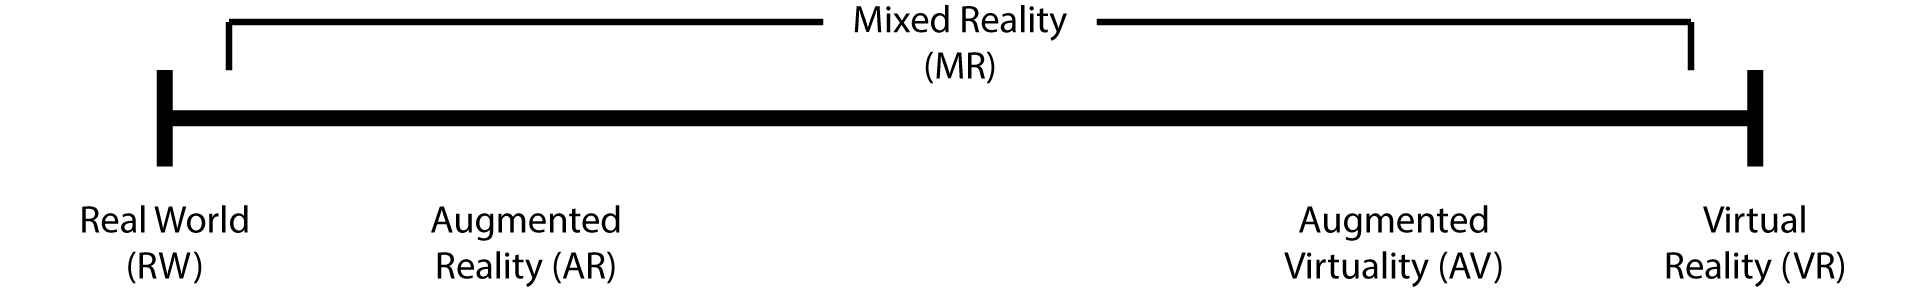
\includegraphics[width=\textwidth]{images/virtuality-continuum-original.png}
		\caption{Milgram \& Kishino's virtuality continuum.}
		\label{virtuality-continuum-original}
	\end{center}
\end{figure}

Of particular importance is to appreciate the distinction between a XR system \& an \textit{augmented reality} (AR) system, as both concepts involve user engagement with both real \& virtual content. Whilst an AR system features a single environment, comprised of the user's RW overlain by some virtual content, with the user perceiving stimuli from this single augmented environment (figure \ref{virtuality-continuum-augmented-reality}), a XR system instead features two discrete environments, one real \& the other virtual, each complete unto itself (figure \ref{virtuality-continuum-cross-reality-1}).

Whilst AR falls within the realms of Mixed Reality (MR), a XR system can be considered as occupying the two extremes of the continuum outwith the MR region. However, XR systems that allow simultaneous interaction with both of their constituent environments blur this definition; using a XR platform such as that discussed in this document, a user can transition between perceiving stimuli from each of these environments (figures \ref{virtuality-continuum-cross-reality-2} \& \ref{virtuality-continuum-cross-reality-3}) in a manner that allows them to engage with each environment without becoming wholly vacant from the other.

\begin{figure}[h]
	\begin{center}
		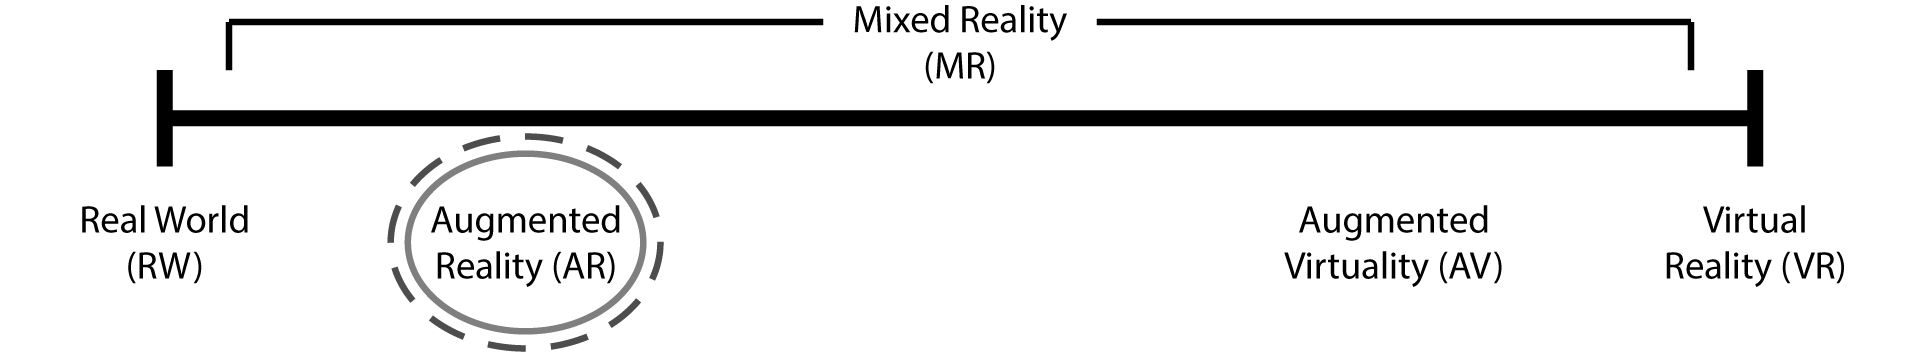
\includegraphics[width=\textwidth]{images/virtuality-continuum-augmented-reality.png}
		\caption{AR visualised using the virtuality continuum.}
		\label{virtuality-continuum-augmented-reality}
	\end{center}
\end{figure}

\begin{figure}[h]
	\begin{center}
		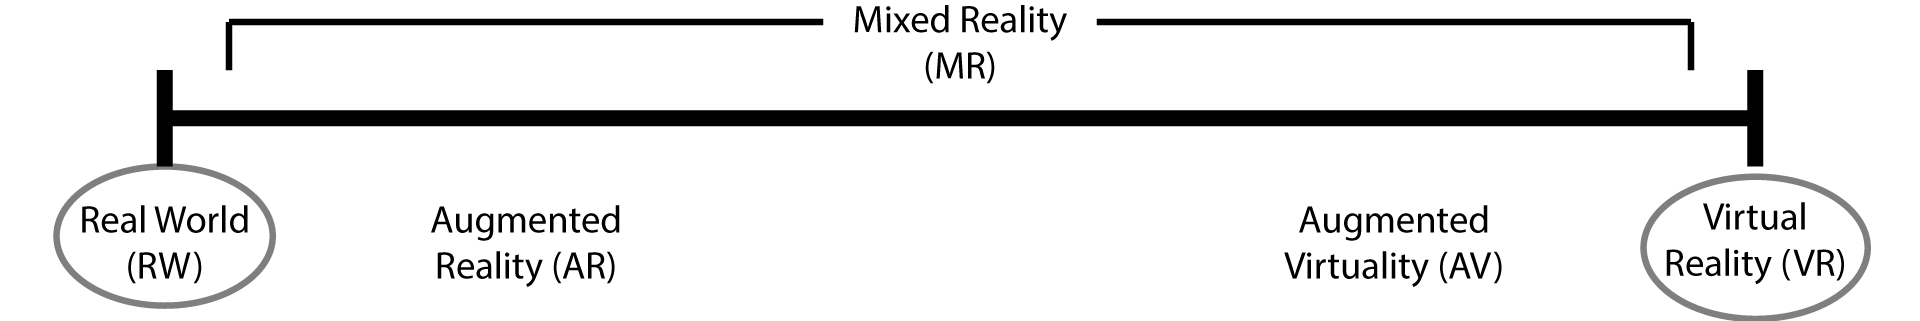
\includegraphics[width=\textwidth]{images/virtuality-continuum-cross-reality-1.png}
		\caption{The two environments that comprise a XR system.}
		\label{virtuality-continuum-cross-reality-1}
	\end{center}
\end{figure}

\begin{figure}[h]
	\begin{center}
		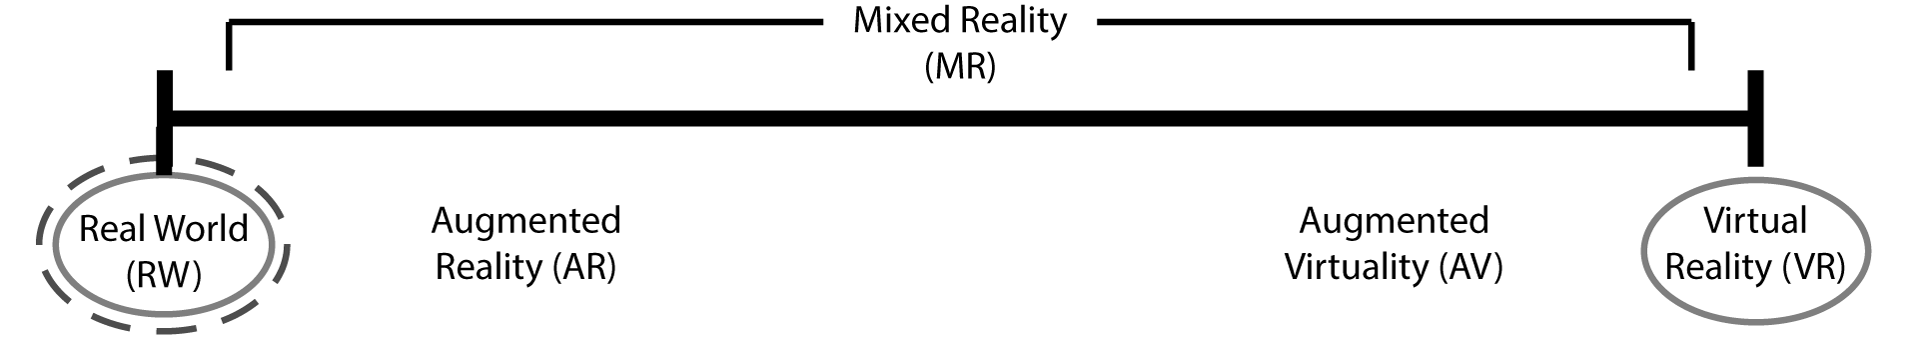
\includegraphics[width=\textwidth]{images/virtuality-continuum-cross-reality-2.png}
		\caption{A XR system with the user attending to RW stimuli.}
		\label{virtuality-continuum-cross-reality-2}
	\end{center}
\end{figure}

\begin{figure}[h]
	\begin{center}
		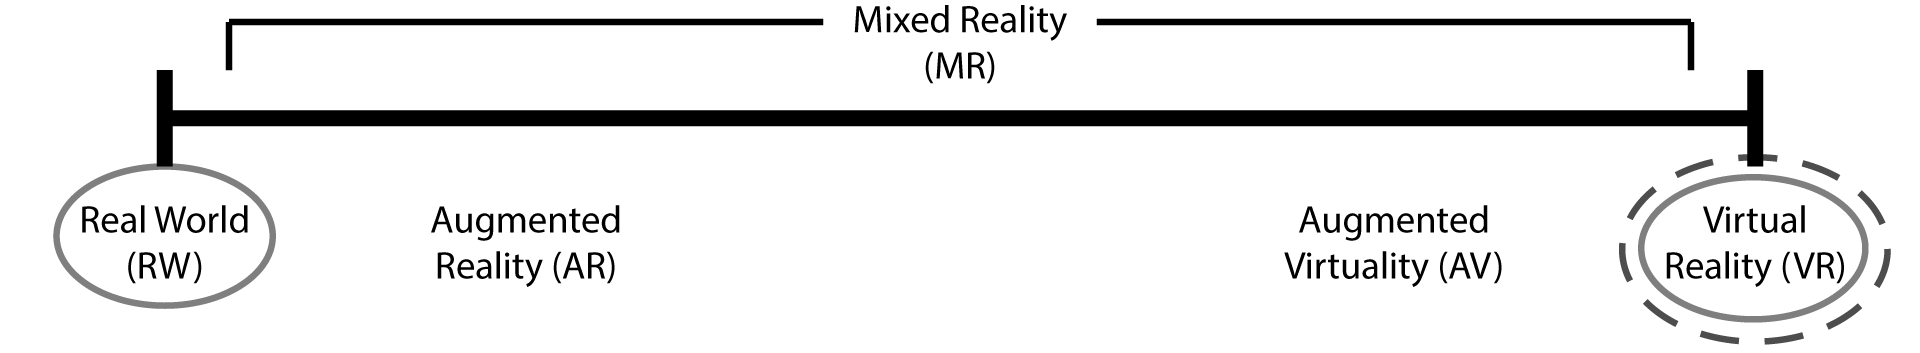
\includegraphics[width=\textwidth]{images/virtuality-continuum-cross-reality-3.png}
		\caption{A XR system with the user attending to VR stimuli.}
		\label{virtuality-continuum-cross-reality-3}
	\end{center}
\end{figure}

\clearpage

%=========================================================================================================
%=========================================================================================================

\section{Position - \textit{Waterworth \& Waterworth}}
\label{waterworth}
\newcommand{\presencefootnote}{\footnote{\textbf{Presence} in this context is defined as a state of heightened perceptual processing of environmental stimuli (\textit{``a psychological focus on direct perceptual processing''}~\cite{Waterworth2001}) accompanied by lessened conceptual reasoning, whether these environmental stimuli originate from a real environment, a virtual environment, a mixed reality environment, or even from multiple discrete environments.}}

\newcommand{\absencefootnote}{\footnote{\textbf{Absence} is defined as \textit{``a psychological focus on \ldots conceptual processing''}~\cite{Waterworth2001}.}}

The virtuality continuum is here considered to be analogous to the \textit{locus of attention} axis of Waterworth \& Waterworth's \textit{three dimensions of virtual experience} model~\cite{Waterworth2001}; the combination of these models is shown by figure \ref{focus-locus-sensus-with-virtuality-continuum}. In this model, locus of attention represents the environment where the stimuli that the user is perceiving originate from; focus of attention represents the balance between conceptual/abstract reasoning \& perceptual/concrete processing, where complex conceptual reasoning results in little attention being paid to processing environmental percepts (whether originating from real or virtual stimuli) thus reducing presence\presencefootnote{} in that environment toward its antithesis $-$ absence\absencefootnote{}; and sensus of attention represents the level of conscious arousal (or `wakefulness'~\cite{Laureys2009}) of the user, whether directed toward percepts originating from real stimuli, virtual stimuli, a mix, or not directed toward any percepts in the case of completely `absent' conceptual reasoning.

\begin{figure}[h]
	\begin{center}
		
\includegraphics[width=0.685\textwidth]{images/focus-locus-sensus-with-virtuality-continuum.png}
		\caption{The combined virtuality continuum/three dimensions of virtual experience model.}
		\label{focus-locus-sensus-with-virtuality-continuum}
	\end{center}	
\end{figure}

%The Sensus Dimension - the importance of being awake in class
%"Even as we sleep dreamlessly..." (example of being 'unconscious' in this regard)

%fourth axis is alterity, between hermeneutics \& embodiment

%=========================================================================================================
%=========================================================================================================

\section{The Case for Mobile XR}

%ARCHEOGUIDE makes the point that AR is good because users are not isolated/completely immersed in a synthetic world - well Mirrorshades allows uers to more fully immerse themselves in a synthetic world, but without becoming isolated in it (eg without becoming ***vacant*** from the real world)

A XR system that presents the user with visual stimuli from both its constituent environments (RW \& VR) allows that user to engage with both real \& virtual content in a manner that is similar to, but has a number of advantages over, a traditional AR system;

\begin{itemize}
	\item the XR system is less critical of registration (the accurate positioning/alignment) between real \& virtual, as the virtual objects are seen as part of a larger virtual environment instead of being rendered atop a view of the real environment;
	\item the XR system can make use of existing VR content without the overhead of decanting/extracting a subset of the virtual components into an AR framework (e.g. manually selecting which objects within the VR environment are to be displayed over the RW environment);
	\item the use of a complete VR environment allows the virtual content to be more encompassing \& immersive, as presenting a complete VR environment allows total control over lighting, shadows, reflections, particle effects, etc. which would be difficult or impossible for an AR platform to render atop a view of a RW environment.
\end{itemize}

Thus, such a XR platform is well suited to situations in which interaction with both real \& virtual visual stimuli is required \& where one or more of the following hold true;

\begin{itemize}
	\item in lieu of accurate registration between real \& virtual, there is a strong focus on the virtual environment's atmosphere \& immersion~\cite{deamicis:gamebased};
	\item there is existing VR content;
	\item the visual differences between real \& virtual environments are so substantial that an AR system would resort to augment (\&/or diminish~\cite{Mann2002}) almost the whole RW view. While AR \textit{``smears an informational coating over real space''}~\cite{Andersen}, XR presents a complete, discrete virtual environment. AR is beneficial where one wishes the juxtaposition of virtual objects upon what is already present in the RW environment, however VR is better suited to situations where one wishes to present a complete virtual alternative.
\end{itemize}

\section{Example Application - Cultural Heritage}
The field of cultural heritage has seen widespread applications of both AR~\cite{Kim2009, Wojciechowski2004, Okura2006, Magnenat-Thalmann2008a, vlahakis:archeoguide, Okura2011, Seo2010, benko:collaborative, Papagiannakis2004, Magnenat-Thalmann7, Papagiannakis2005, Papagiannakis2007, Papagiannakis2009, Taketomi2011, walczak:applications} \& VR~\cite{deamicis:gamebased, roussou:photorealism, cabral:x3dexperience, Roussou2002, Christou2006, willmott:largecomplex, Tzortzaki2002}. AR has been used to add artefacts, actors \& reconstructed architecture to views of present day sites that bear traces of their original status, whilst VR has been used to host more complete reconstructions of entire buildings \& settlements for interaction via screen, HMD \& CAVE, including where the present day site bears no evidence of the past status or is inaccessible for some reason (due to latter development, change in landscape, etc.).

In situations where VR content exists in cultural heritage contexts, it is experienced from a static position that causes both spatial \& temporal separation from the RW location that it relates to; in order to perform comparisons between RW \& VR content, users must interact with one \& \textit{subsequently} the other. A mobile XR platform will allow VR content in cultural heritage contexts to be experienced in tandem with the real site (where accessible), combining the immediate juxtaposition of real \& virtual content of AR with the immersive \& atmospheric qualities of HMD based VR, all without requiring alterations to the VR content (for example to make it compatible with an AR framework).

%fixed/anchored AR interface~\cite{Weng2012}

\pagebreak

\section{Case Study - St Salvator's Chapel}
Founded in 1450 but internally stripped of its medieval fittings during the Protestant Reformation (1517 - 1648), St Salvator's chapel in St Andrews looks markedly different in the present day than it did upon its completion. An existing VR reconstruction of the chapel as it stood in the period 1450-1460 \& the marked differences between the internal appearance of the VR building \& the current building (including the replacement of the original stone roof with a wooden one \& drastically different dividing of the internal space) make this chapel an ideal candidate within the context of cultural heritage for a mobile XR system to be applied. Figure \ref{sallies_layout} shows the 1450-1460 layout of the chapel (including the paths that the IPS has been prepared upon).

\begin{figure}[h]
	\begin{center}
		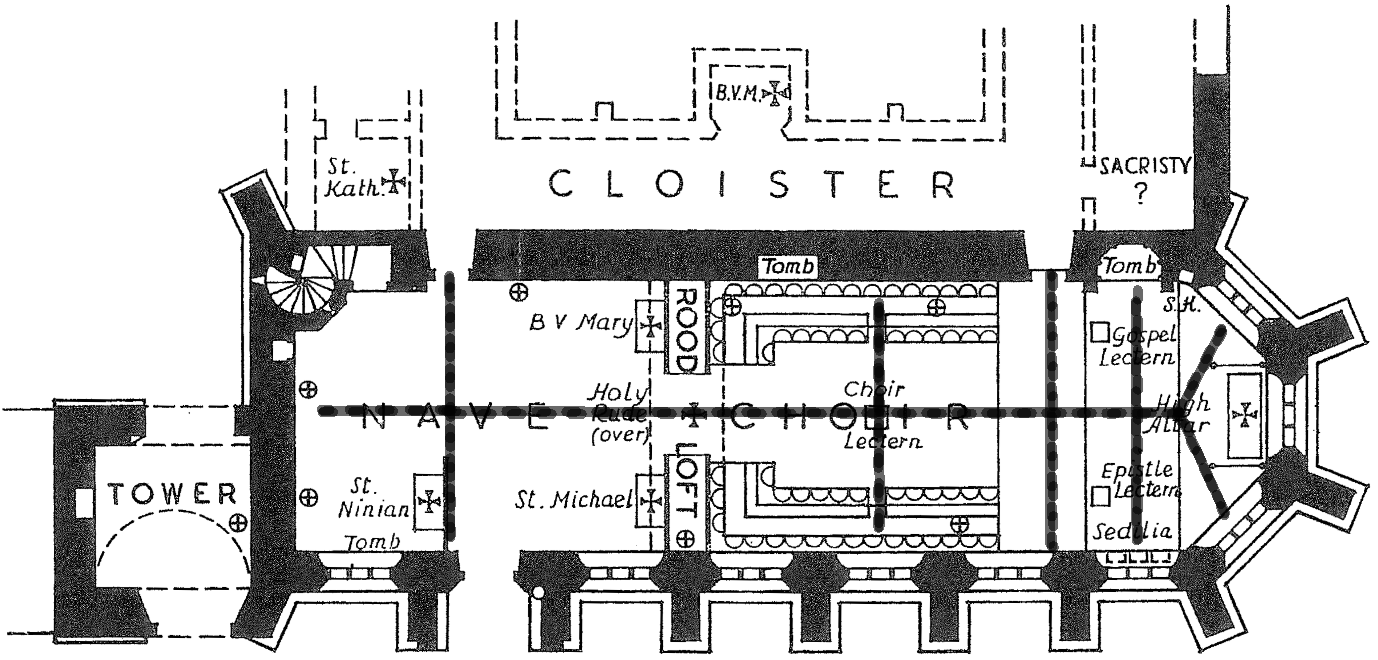
\includegraphics[width=0.7\textwidth]{images/sallies_layout.png}
		\caption{Floor plan of St Salvator's chapel, with IPS routes.}
		\label{sallies_layout}
	\end{center}
\end{figure}

\clearpage

%=========================================================================================================
%=========================================================================================================

\chapter{The Mirrorshades Platform}
Figure \ref{systemarchitecture} presents a high level architectural overview of our mobile XR platform, dubbed Mirrorshades\footnote{\textbf{Mirrorshades: The Cyberpunk Anthology} (1986) is a defining cyberpunk short story collection, edited by Bruce Sterling.}.

\begin{figure}[h]
	\thispagestyle{empty}
	\begin{center}
		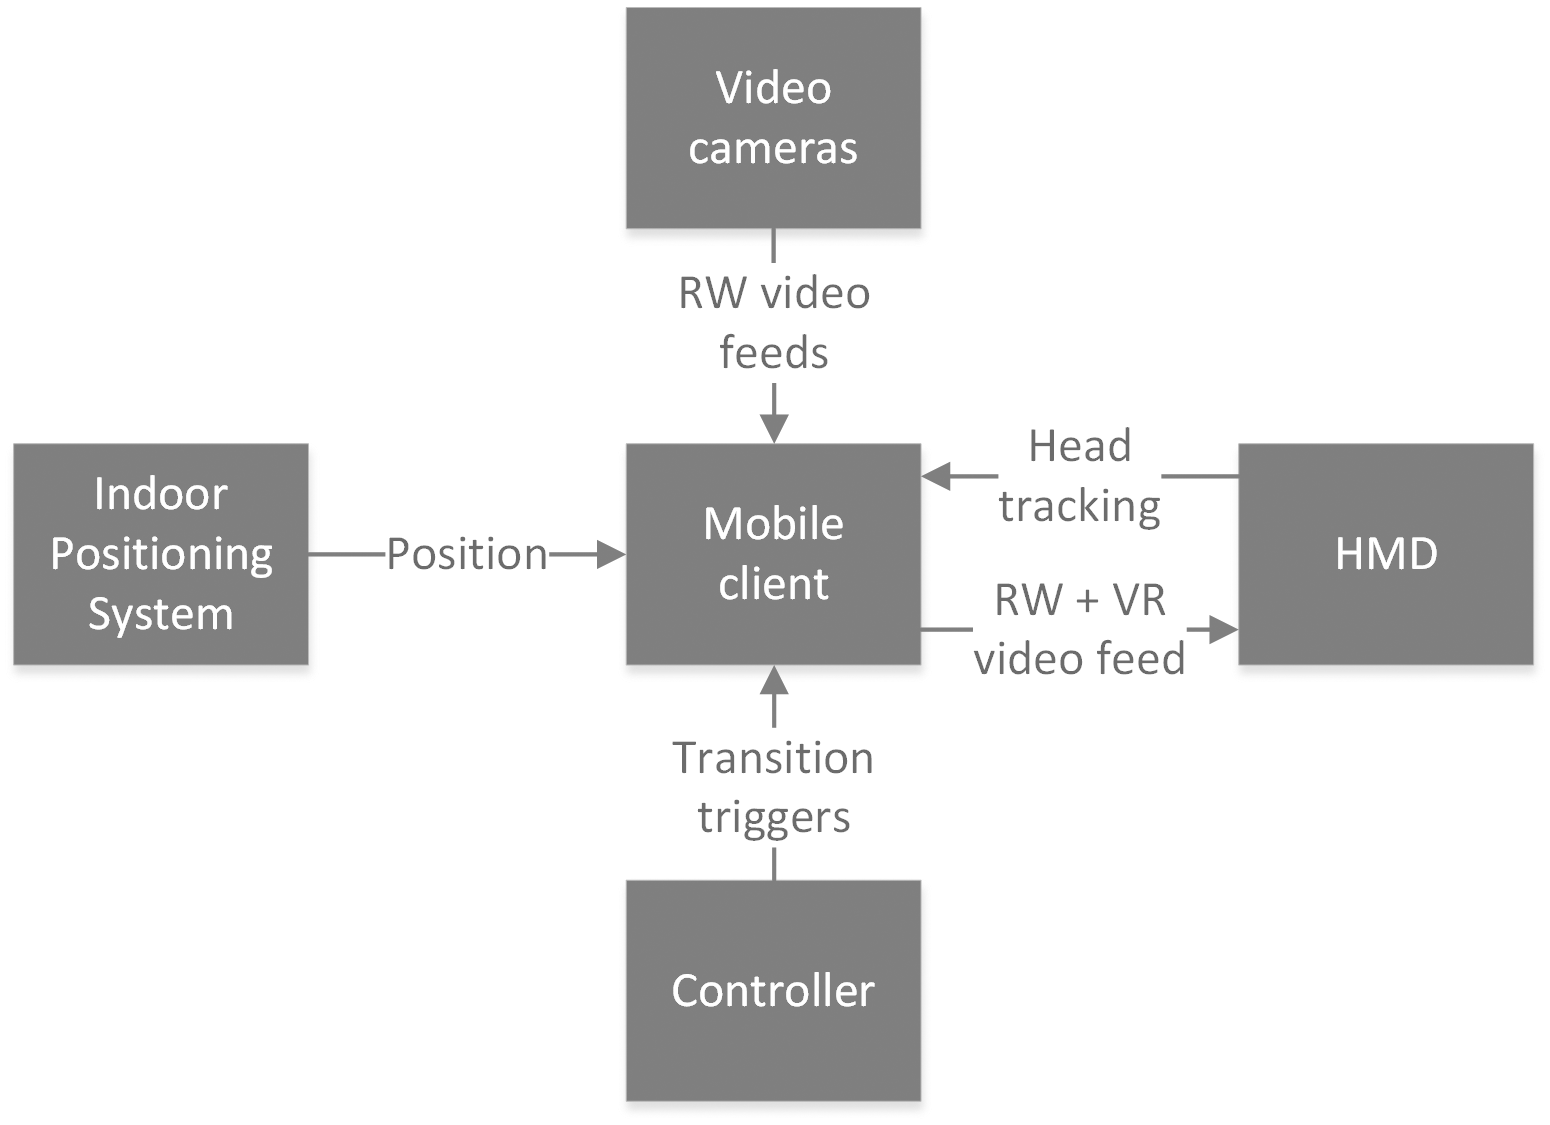
\includegraphics[width=.5\linewidth]{images/system-architecture.png}
		\caption{Overview of the Mirrorshades platform.}
		\label{systemarchitecture}
	\end{center}
\end{figure}

%=========================================================================================================
%=========================================================================================================

\section{Implementation}
Figure \ref{experimentalimplementation} presents an overview of the implementation of the Mirrorshades platform design for use in the chapel investigations.

\begin{figure}[h]
	\thispagestyle{empty}
	\begin{center}
		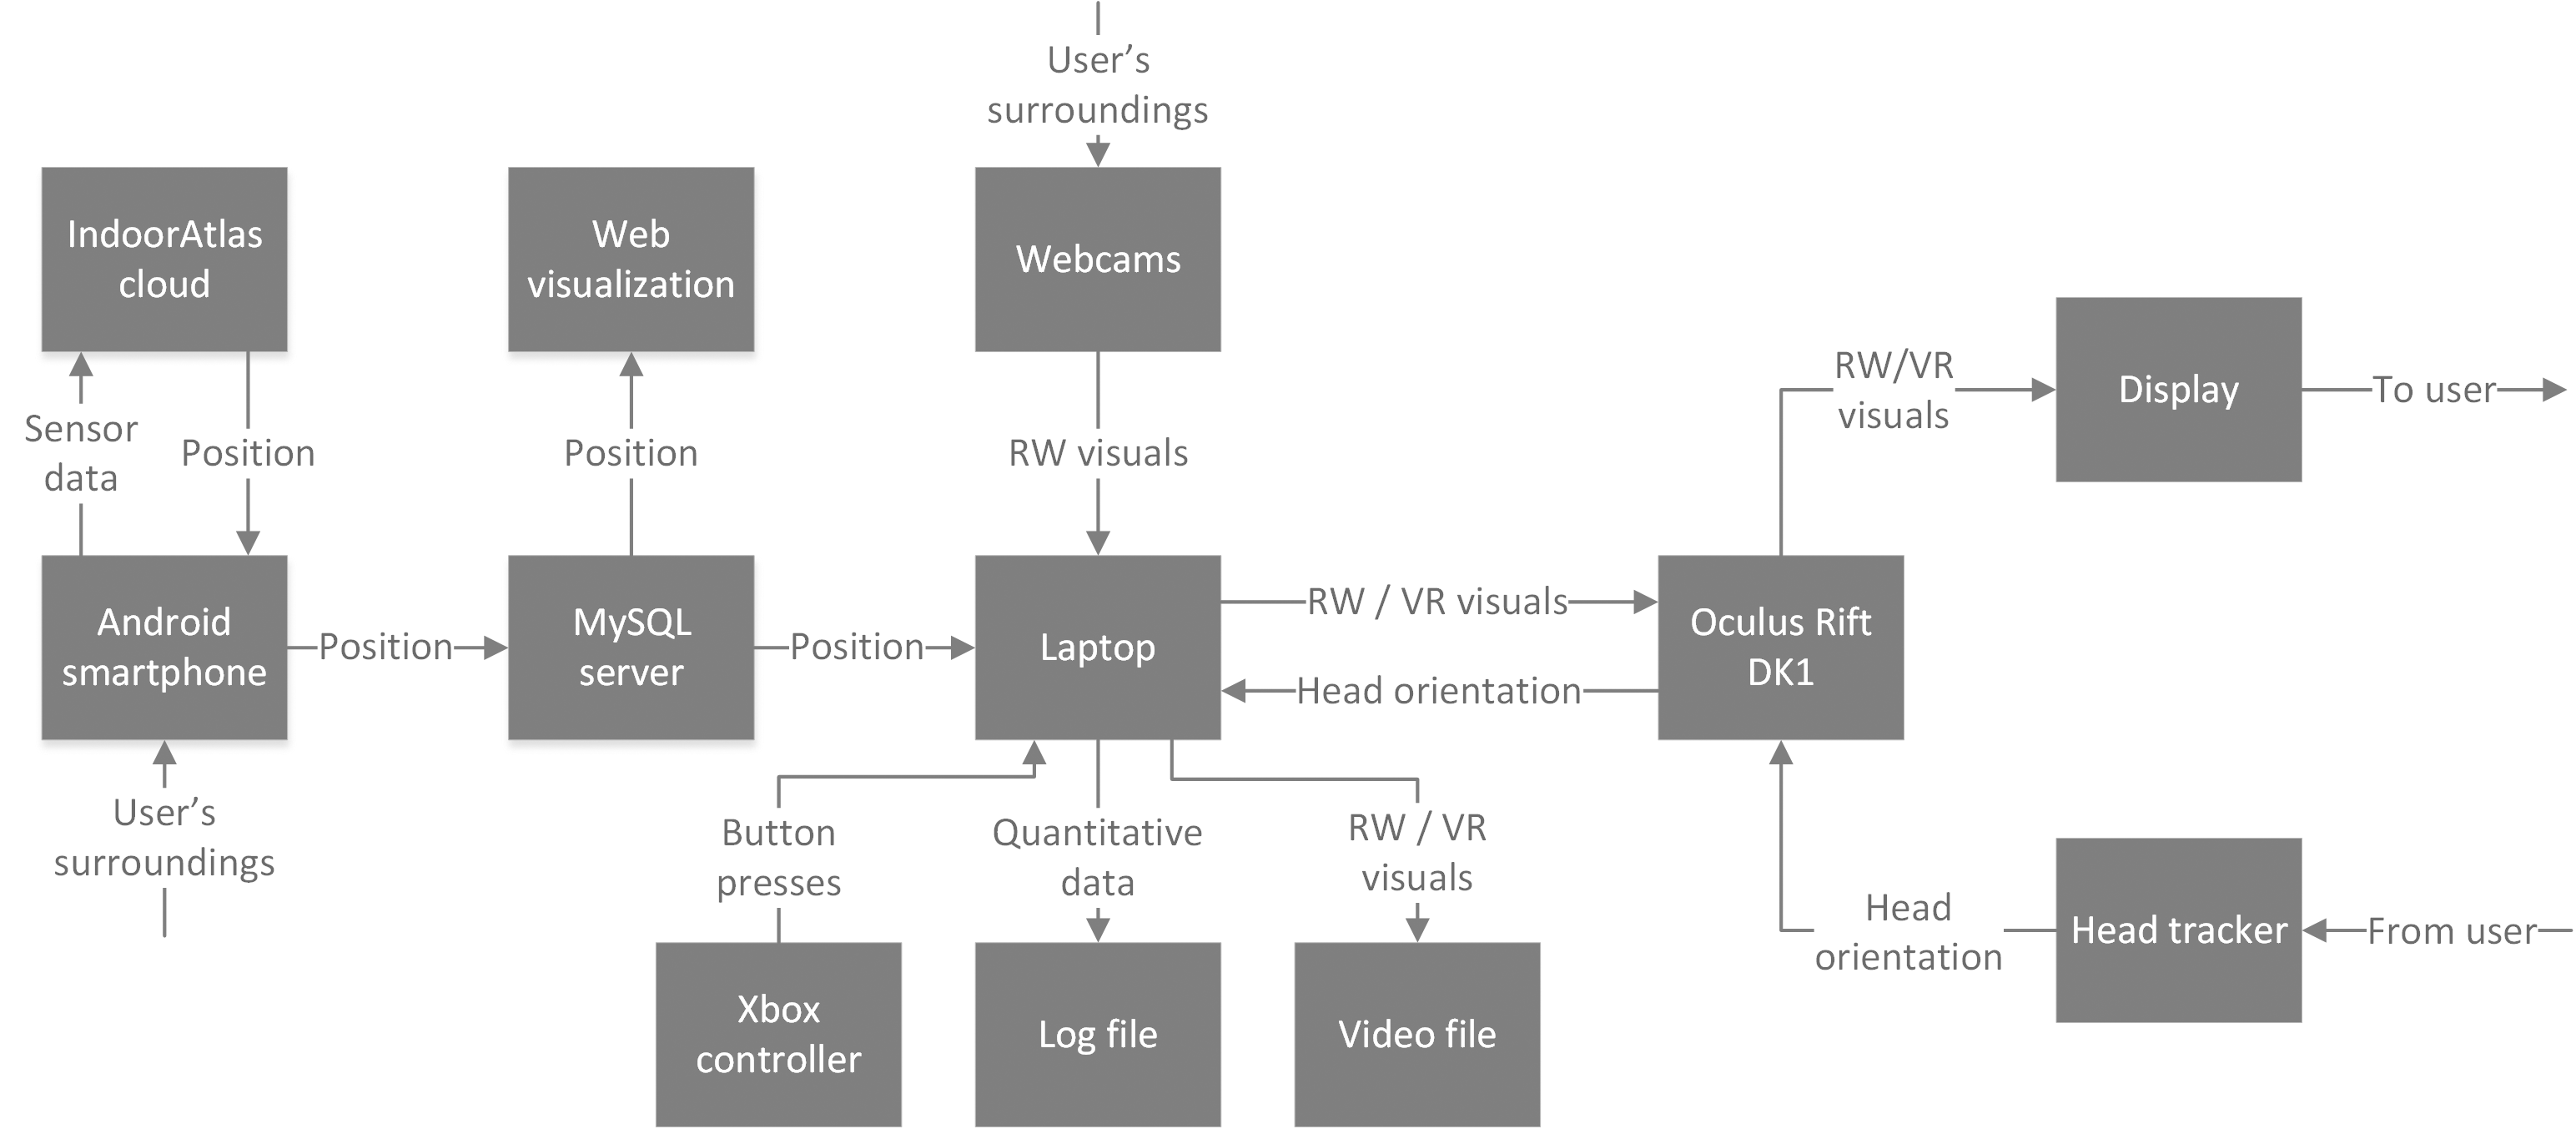
\includegraphics[width=.925\linewidth]{images/experimental-implementation.png}
		\caption{Implementation of Mirrorshades platform.}
		\label{experimentalimplementation}
	\end{center}
\end{figure}

\section{Hardware Components}
The hardware of the implementation comprises;

\begin{itemize}
	\item an Oculus Rift DK1 HMD, including a 9-axis (3dof rotational) head tracker sampling at 1000Hz \& mounted with a stereo camera solution comprising 2x Logitech C310 webcams modified with M12 lens mounts \& 2.1mm lenses to provide approximately 87 degrees horizontal FOV of the RW environment (see figure \ref{rift});
	\item a USB battery pack, to power the HMD;
	\item a small laptop computer, with an Intel i7-3632QM processor, Nvidia GT 650M graphics card \& 16GiB system memory;
	\item an Android smartphone, running Android 4.4.4;
	\item an Xbox 360 wireless controller, with USB receiver.
\end{itemize}

\begin{figure}[h]
	\begin{center}
		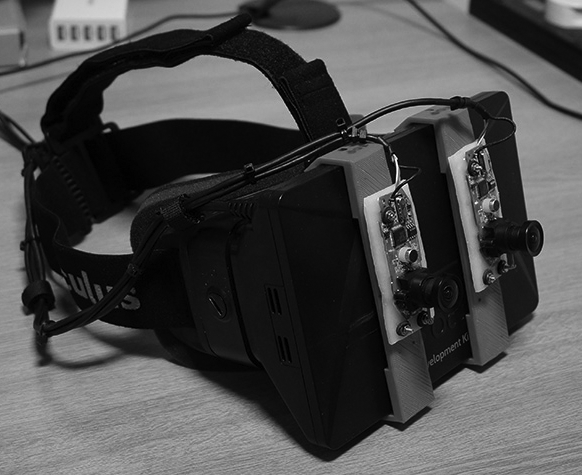
\includegraphics[width=0.6\textwidth]{images/rift.png}
		\caption{HMD with stereo camera solution.}
		\label{rift}
	\end{center}
\end{figure}

\section{Software Components}
The software of the implementation comprises;

\begin{itemize}
	\item an Android application that runs on the smartphone, determines the location of the phone within the building that it is in using the IndoorAtlas IPS~\cite{IndoorAtlasLtd.2012} (figure \ref{sallies_layout} shows the paths within the chapel upon which the IPS has been configured) \& submits these location data via PHP to a database server;
	\item a MySQL database server that stores location data for the phone \& allows these data to be accessed both by the Unity application running upon the laptop \& by a web visualisation;
	\item a Unity application that runs on the laptop.
\end{itemize}

\section{Integration of Components}
The Unity application hosts the VR representation of the chapel \& takes in feeds from both webcams, the HMD head tracker \& the Xbox controller. It also polls the database server for the most recent position data. All of these inputs are combined together to form the visual output for the HMD to display to the user.

As the user moves their head, the visuals that are presented to them upon the HMD's display change accordingly; the RW visuals change due to the webcams being physically fixed to the HMD \& the VR visuals change due to data from the head tracker being used to change the orientation of the in game `cameras' accordingly.

As the user changes their position by walking, the visuals that are presented to them upon the HMD's display also change accordingly; again the RW visuals change due to the webcams' position upon the HMD whilst the VR visuals change due to the user's position, as reported by the smartphone \& the IndoorAtlas solution, being used to move the position of the in game cameras to the equivalent position within the VR representation.

As the user presses buttons or pulls triggers upon the Xbox controller, the visuals that are presented to them upon the HMD's display transition between RW \& VR in different styles depending upon which button/trigger was activated.

%=========================================================================================================
%=========================================================================================================

\chapter{Investigation 1 - The Case for Mobile XR}
\label{investigation1}
This first investigation will compare interaction with the RW \& VR chapel using Mirrorshades to interaction with the same content separately, the latter being the approach usually adopted for dissemination of VR content in cultural heritage contexts. Participants will complete a task that will promote active comparison \& contrast of the RW \& VR environments, whilst navigating a set route. This investigation will gauge through experimentation whether the Mirrorshades platform provides any value over the traditional manner in which the same VR content might be disseminated at a cultural heritage site.

%spatial \& temporal separation

\section{Setting \& Task}
This investigation comprises two phases;

\begin{enumerate}
	\item Participants will experience the RW \& VR chapels separately. They will navigate the VR chapel from a stationary position, as one might expect to see a VR installation at a cultural heritage site, using the Xbox controller to move around the VR environment observed via the HMD. The HMD will obscure their view of the RW chapel around them. Subsequently, they will navigate the RW chapel without the HMD or any associated equipment.
	\item Participants will experience the RW \& VR chapels in tandem using the Mirrorshades platform. They will wear the HMD, holding the Xbox controller in their right hand \& the smartphone in their left, with the laptop \& battery pack in a satchel worn over one shoulder. One style of transition will be available to the participants during this phase.
\end{enumerate}

In all 3 scenarios (phase 1 VR, phase 1 RW, phase 2 RW + VR) the participant will navigate the same route \& will be instructed to identify a particular feature/object within the chapel (see figures \ref{pews} \& \ref{ceiling}), situated somewhere upon the set route, that differs in its appearance \&/or location between the RW \& VR chapels. The order in which the two phases are completed will be randomised between participants, as will the features that they are told to observe in each phase. Participants will have a maximum length of time to navigate the route \& will be allowed to stop before this time has elapsed should they wish.

%\begin{figure}[h]
%	\begin{center}
%		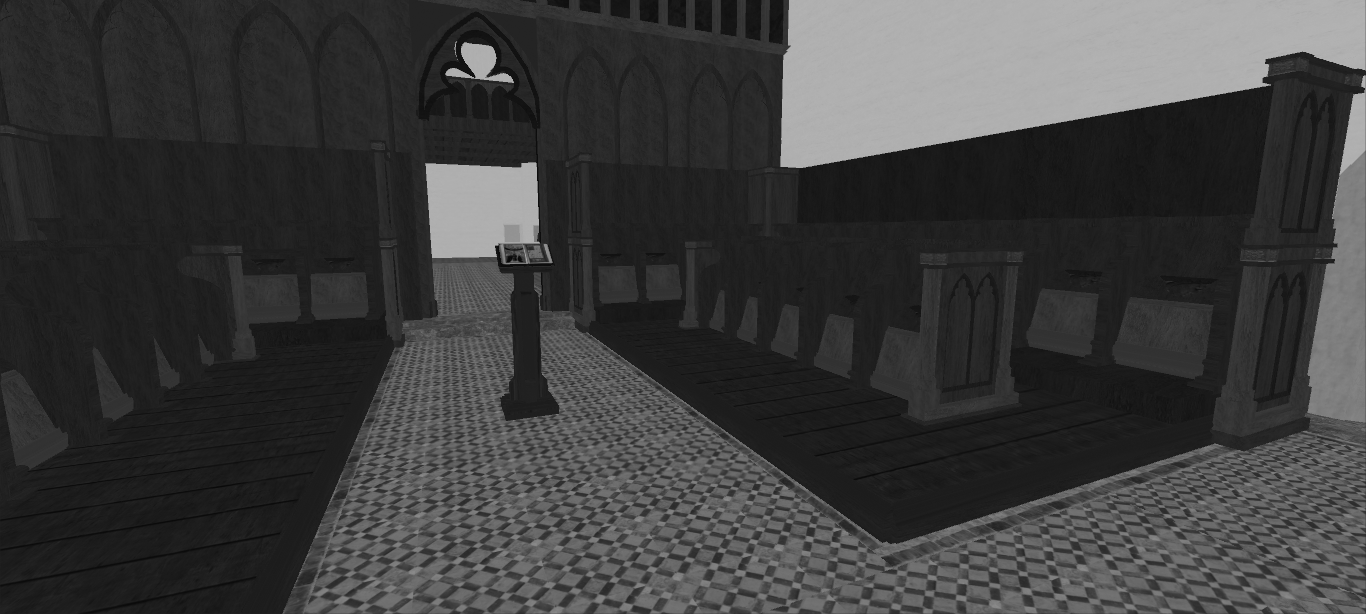
\includegraphics[width=0.7\textwidth]{images/pews.png}
%		\caption{Chapel pews, greater in number in present day.}
%		\label{pews}
%	\end{center}	
%\end{figure}

%\begin{figure}[h]
%	\begin{center}
%		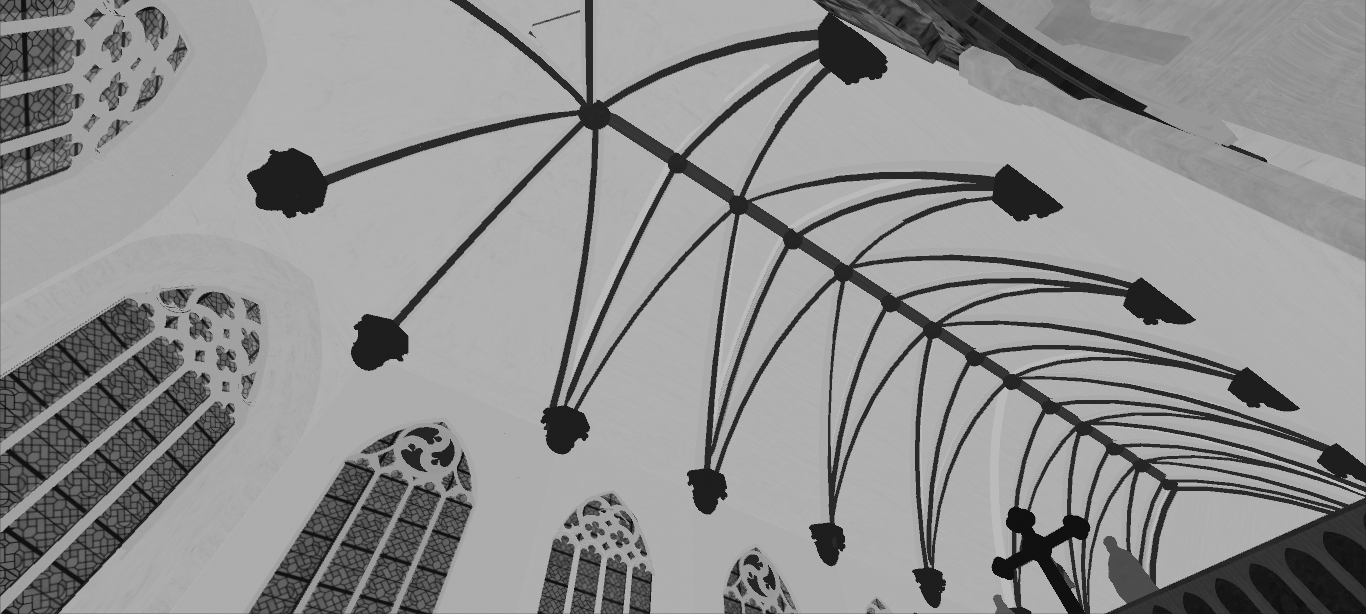
\includegraphics[width=0.7\textwidth]{images/ceiling.png}
%		\caption{Chapel ceiling, different construction in present day.}
%		\label{ceiling}
%	\end{center}	
%\end{figure}

%\begin{figure}[h]
%	\begin{center}
%		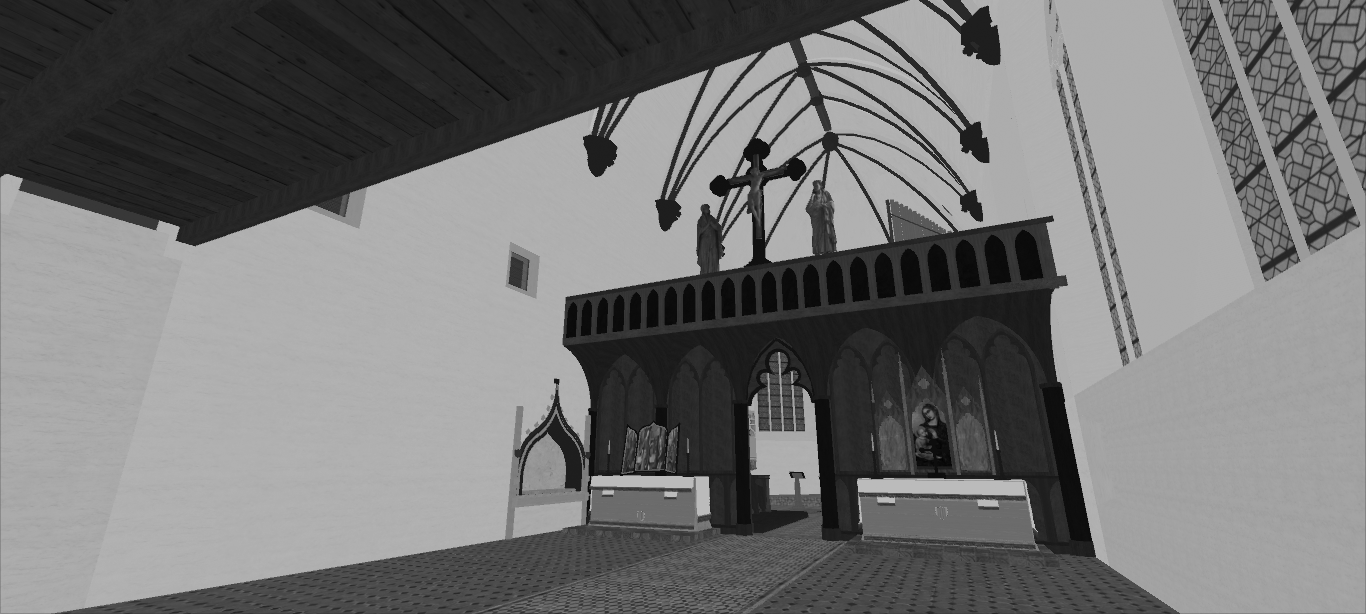
\includegraphics[width=0.7\textwidth]{images/division.png}
%		\caption{Division of the internal space of the chapel, different position in present day.}
%		\label{division}
%	\end{center}	
%\end{figure}

%rows/number of pews
%position of dividing wall
%colour/construction of ceiling
%number/position of lecterns

\section{Evaluation Techniques}
Evaluation will be performed via a short structured interview \& completion of the System Usability Scale (SUS)~\cite{Brooke1996}.

%\begin{itemize}
%	\item (General) Which did you prefer?
%	\item Which did you think made it easier for you to perform comparisons between real \& virtual?
%	\item Which was more rewarding (if you were visiting the site genuinely)?
%	\item Which gave a better understanding of the changes that have been effected to the building?
%	\item Did you notice/discover anything in one scenario that you didn't in the other?
%	\item Etc.
%\end{itemize}

\section{Hypothesis}
SUS responses are expected to average fairly low due to the cumbersome nature of the platform's implementation. Participants who are able to overcome this cumbersomeness are expected to respond favourably to the platform, with those who cannot overcome it responding in favour of the traditional `separate' approach instead.

%=========================================================================================================
%=========================================================================================================

\chapter{Investigation 2 - Informing Mobile XR Implementation}

\newcommand{\breakinpresencefootnote}{\footnote{The definition of \textbf{break in presence} adopted herein is the second from Waterworth \& Waterworth~\cite{Waterworth2001} (p205): a movement along the focus axis away from presence in the real or a virtual environment \& toward absence. This differs to Slater \& Steed's original definition in~\cite{Slater2000} as they considered presence only in terms of attending to stimuli from a virtual environment, with a break in presence as a Gestalt switch to instead attending to stimuli from the real environment. Waterworth \& Waterworth's model considers presence in terms of attending to stimuli from either the real \textit{or a virtual} environment, with a break in presence representing absence in the sense of heightened conceptual load \& the resultant reduced perceptual processing of environmental stimuli originating from \textit{either} the real or a virtual environment. This definition better fits the situation invoked by the Mirrorshades platform, which is concerned with intentionally \& willingly switching engagement between stimuli from both real \& virtual environments, rather than engaging with stimuli from only a virtual environment in a scenario where stimuli from the real environment are considered a `distraction'.}}

The novel aspect of the Mirrorshades platform is the ability it imparts upon its user to switch their locus of attention between equivalent vantage points in RW \& VR environments whilst walking around. This is achieved by the user performing transitions between RW visual stimuli \& VR visual stimuli, both presented via their HMD. This extends existing XR research by allowing the user to engage with the visual stimuli of the VR component of a XR system from any position \& at any time.

In order to achieve the highest quality of experience with this style of interaction with XR systems, it is vital to determine how best to implement these transitions; that is, to mitigate the increased cognitive load (manifesting as increased conceptual reasoning \& reduced perceptual processing, see section \ref{waterworth}) required to comprehend these transitions, as this increased cognitive load will detract from engagement with the environments \& reduce the user's willingness to perform these transitions.

Whilst some researchers support the notion that in systems where more than one environment competes for the user's locus of attention there is an `all or nothing' Gestalt switch between awareness of one environment \& the other~\cite{Slater2002}, which would result in a substantial increase in cognitive load upon each transition, Mirrorshades has been developed in support of the contrary opinion; that switching locus of attention from the stimuli of one environment to those of another does not completely overrule the user's awareness of the former, that both environments can be perceived at the same time (albeit one to a lesser extent)~\cite{Ijsselsteijn2001} \& that when engaging with VR content a user's focus can even be said to typically be \textit{shared} between VR \& RW~\cite{Waterworth2001}.

This latter position is particularly apt for situations wherein the RW \& VR environments share the same fundamental layout \& dimensions, as those in a XR system often do, as the inherent familiarity between the two environments reduces the cognitive load associated with transitioning between them. Furthermore, the notion of experience of presence as changing continually from moment-to-moment~\cite{Heeter2003, Ijsselsteijn1998} lends confidence to the successful mitigation of the cognitive load associated with these transitions to manageable levels. One might even liken this `switching' between RW \& VR to the `cycling through' behaviour observed in users of virtual communities, which stemmed from the `window' concept of modern computer operating systems~\cite{Turkle2004}.

However, no matter how smooth the transition the process is expected to always result in some heightened cognitive load, a temporary \textit{break in presence}\breakinpresencefootnote{} (BIP), as the user comes to terms with the new environment presented to them \& comprehends its relation to the other environment that they were just perceiving.

%\section{Transitions}
Transitions can be performed in multiple different manners \& it is hypothesized that users will prefer different styles of transition in different situations, surroundings \& scenarios (where `preference' toward a particular style of transition is expected to correlate strongly with a less severe BIP being experienced upon its execution).

To this end, several different transition methods have been developed \& this investigation will endeavour to identify \& quantify preferences toward them, to infer which approaches to transitioning between RW \& VR visual stimuli are more or less appropriate for the different situations that arise where a platform like Mirrorshades may be deployed. In particular, it is hypothesized that there will be a strong correlation between participant movement (or lack thereof) \& choice of particular transition style.

\section{Transitions using the Combined Model}
Visualised using the combined model (see section \ref{waterworth}) as figure \ref{focus-locus-sensus-with-virtuality-continuum-with-transition}, these transitions are an oscillation along the locus axis, between a RW environment at one position \& a VR environment at the other.

Heightened cognitive load required to comprehend a transition is a temporary movement upon the focus axis from presence toward absence (a BIP). With the ability of a wide FOV, stereoscopic 3D, head-tracked HMD to produce immersive VR visual stimuli that require fairly limited cognitive processing \& our inherent ability to engage with our RW surroundings without significant cognitive load, focus is expected to be high (toward the presence extremum) when attending to stimuli from either RW or VR.

Sensus is expected to be largely task dependent, however when performing a task that involves actively engaging with the visual stimuli from either/both of RW or VR it is expected to be high (toward the conscious extremum). Upon triggering a transition, sensus is expected to increase, as the user centres their attention upon relating the visual stimuli from the new environment to those they were just perceiving from the other environment

%Whilst continued exposure to the platform is expected to reduce the severity of the BIPs, mitigating their severity from the outset (reducing the displacement from the presence extremum downwards toward absence) through informed execution of the transitions between RW \& VR is believed to be important to the overall quality of experience that users receive.

%absent-mindedness - caused by increased attention toward a single object of focus (hyperfocus, eg the object of focus is the switch)
% or caused by distraction (again, the switch)

%\clearpage

%\vspace{12mm}

%\begin{figure}[h]
%	\begin{center}
%		
\includegraphics[width=0.7\textwidth]{images/focus-locus-sensus-with-virtuality-continuum-with-transition.png}
%		\caption{Operation of the Mirrorshades platform represented upon the combined model.}
%		\label{focus-locus-sensus-with-virtuality-continuum-with-transition}
%	\end{center}	
%\end{figure}

\begin{figure}[h]
	\begin{center}
		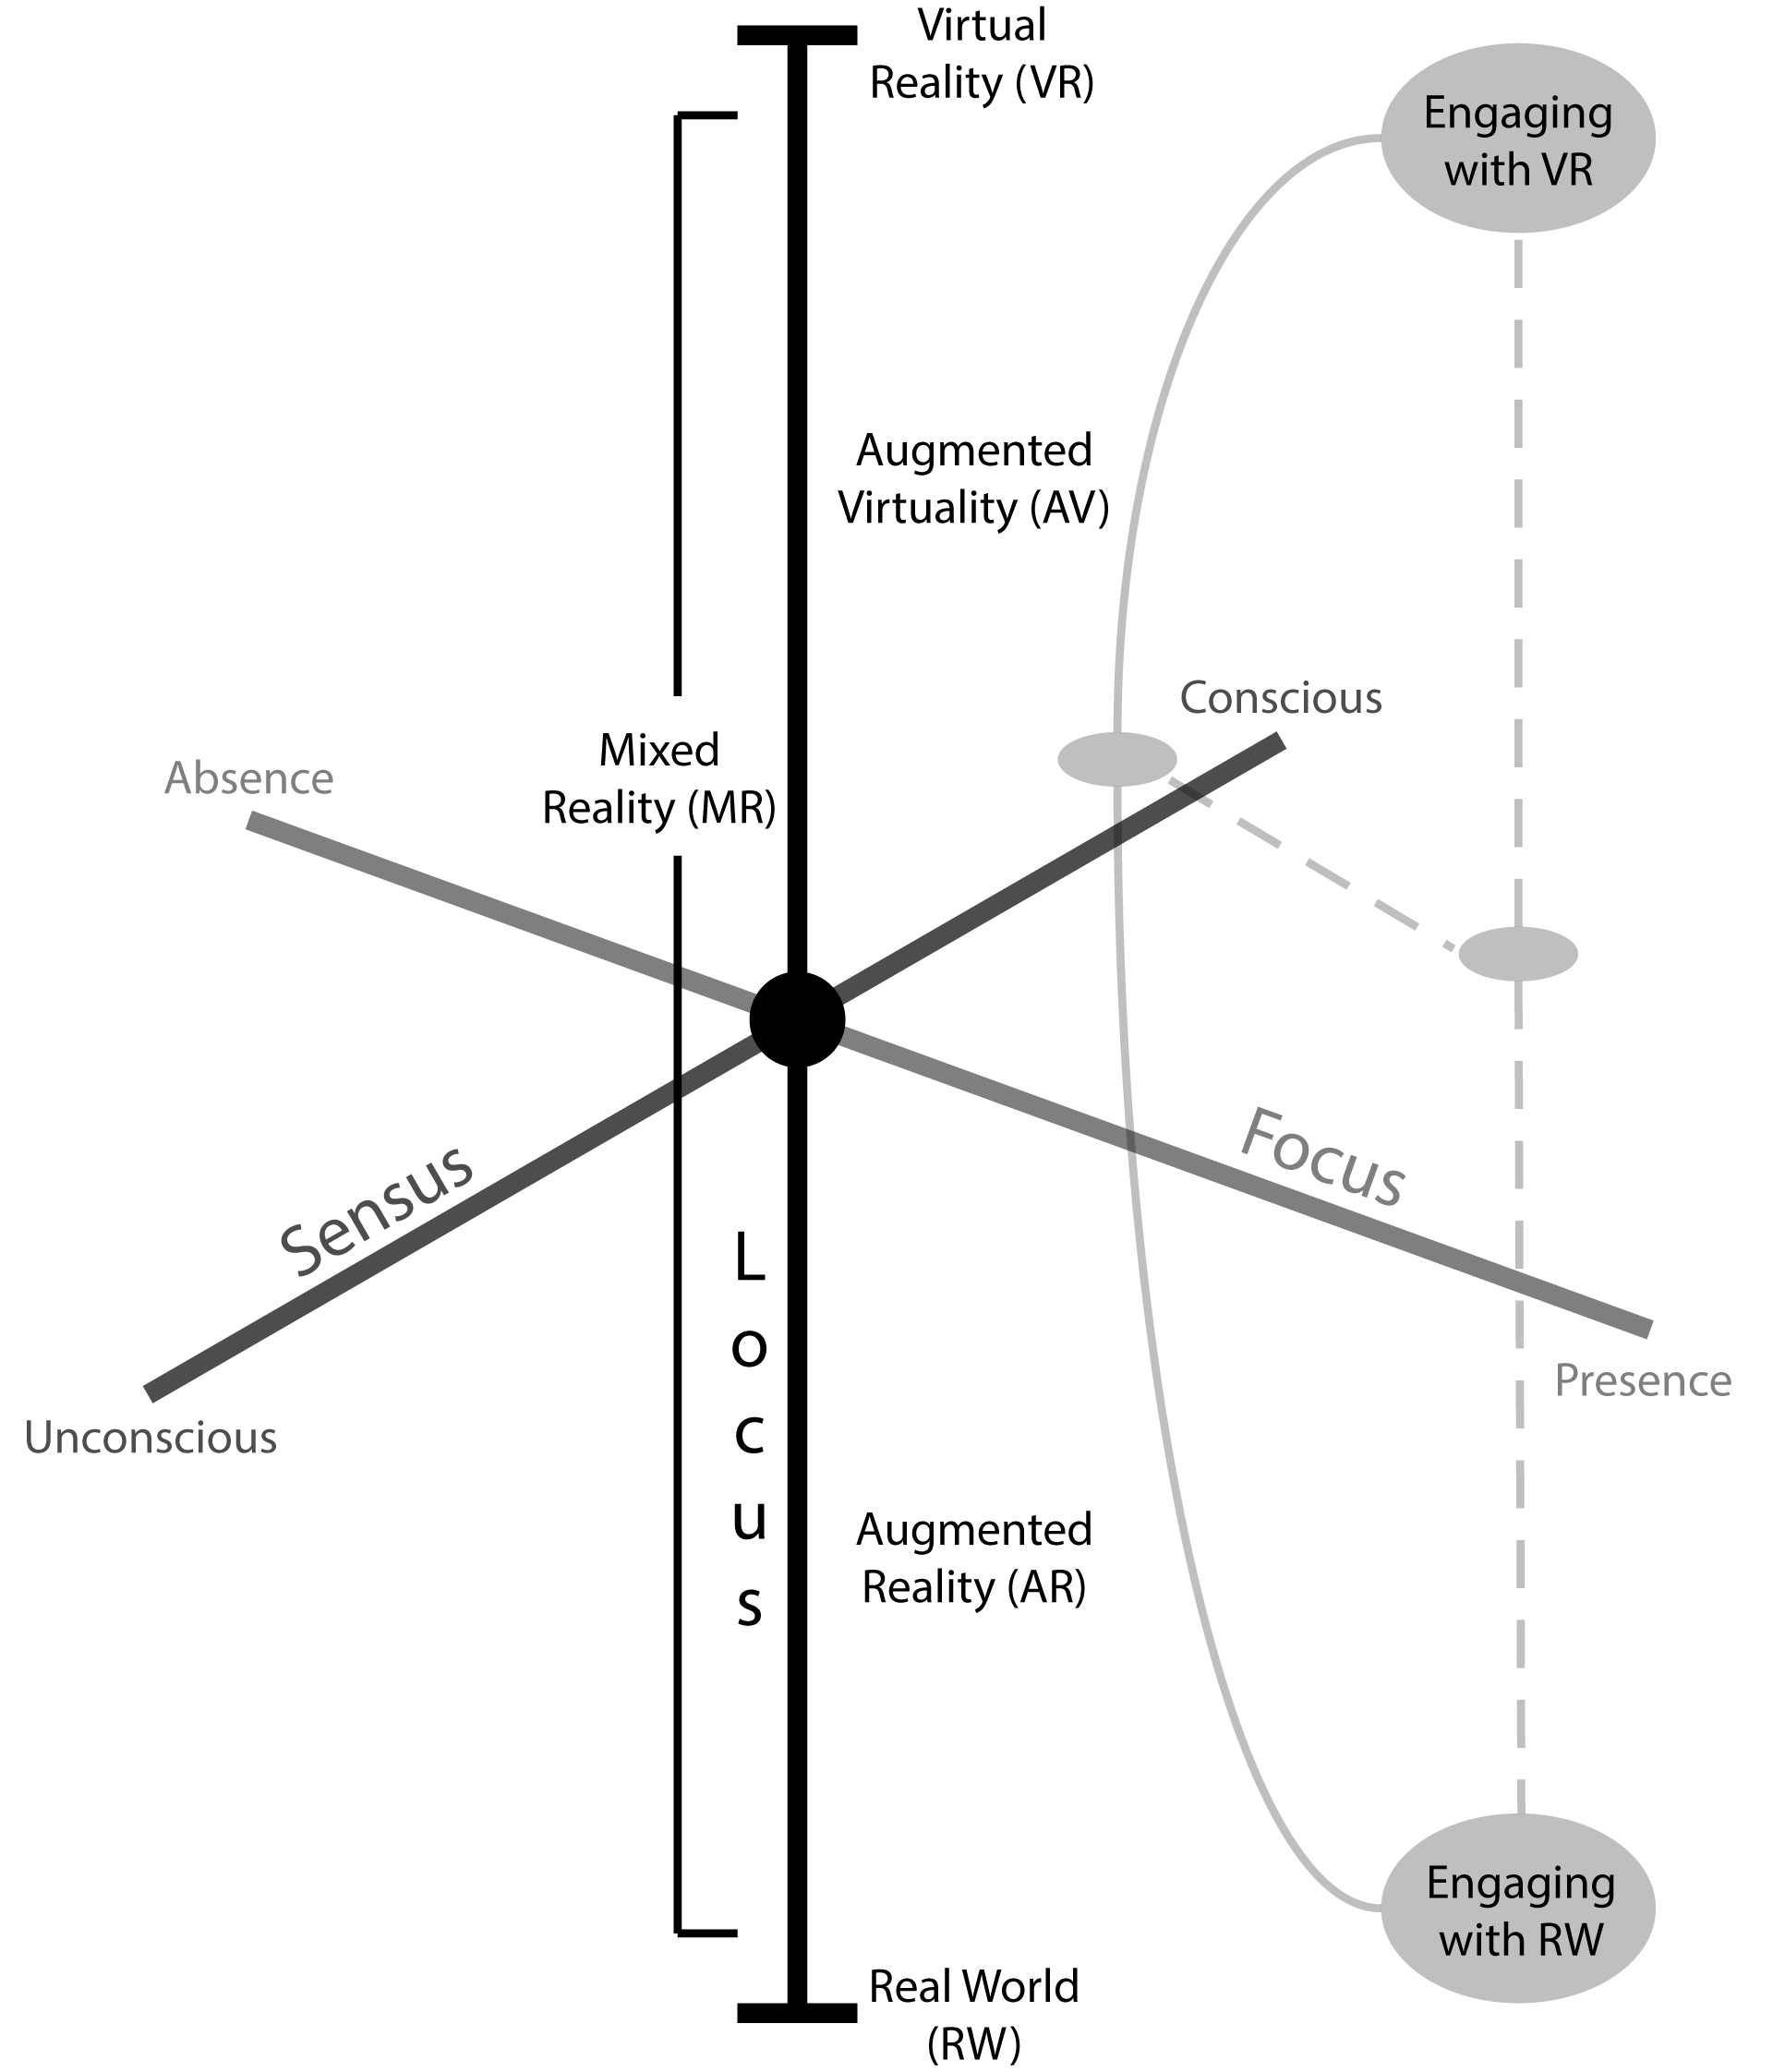
\includegraphics[width=0.7\textwidth]{images/focus-locus-sensus-with-virtuality-continuum-with-transition-updated.png}
		\caption{Operation of the Mirrorshades platform represented upon the combined model.}
		\label{focus-locus-sensus-with-virtuality-continuum-with-transition}
	\end{center}	
\end{figure}

\section{Transition Methods}
Attending to visual stimuli from the RW environment via the webcams is required for the user to safely move around. Delay in the IPS reporting their position \& inaccuracies in these position data (see figure \ref{jack-cole-splodges} for a set of example position data) mean that moving around while attending only to visual stimuli from the VR environment would not be safe for the user, even with unchanging RW obstacles with perfectly accurate representations in the VR environment. Furthermore it is actually likely that RW obstacles will not have equivalent VR representations, such as in a scenario where XR is used to compare \& contrast changes to a building's interior over extended periods of time (such as with the chapel investigations).

\begin{figure}[h]
	\begin{center}
		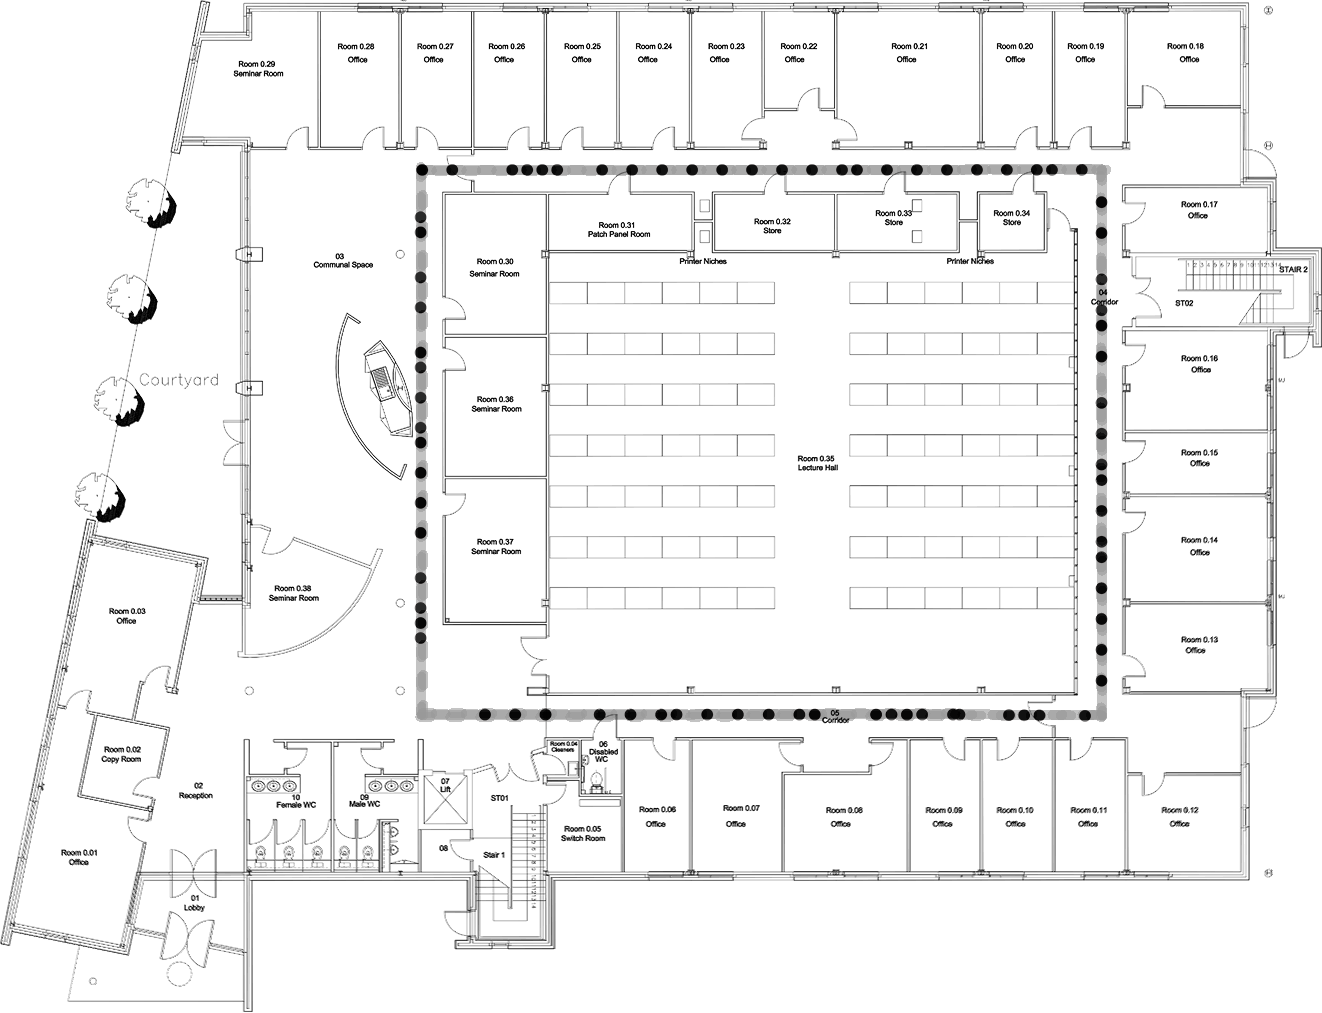
\includegraphics[width=0.7\textwidth]{images/jack-cole-splodges-black.png}
		\caption{Positions (black circles) reported whilst walking a slow lap ($<1$ms$^{-1}$, following gray path) of a departmental building. The building is approximately 40m wide by 30m tall.}
		\label{jack-cole-splodges}
	\end{center}
\end{figure}

Thus the HMD displays the feeds from the webcams as default \& the user must trigger transitions to view the VR environment by pressing a button or pulling a trigger on the controller. Releasing the button/trigger causes the webcam feeds to be displayed again.

\clearpage

\subsection{Hard switch}
\label{sub-hardswitch}
The user presses \& holds the \texttt{[A]} button on the controller to switch the visual stimuli displayed by the HMD from RW to VR. When the \texttt{[A]} button is released, the visual stimuli displayed by the HMD switch back from VR to RW. This is a `hard' or `immediate' switch with no fading or transition effect. Figure \ref{scenario1} illustrates this scenario.

\begin{figure}[h]
	\begin{center}
		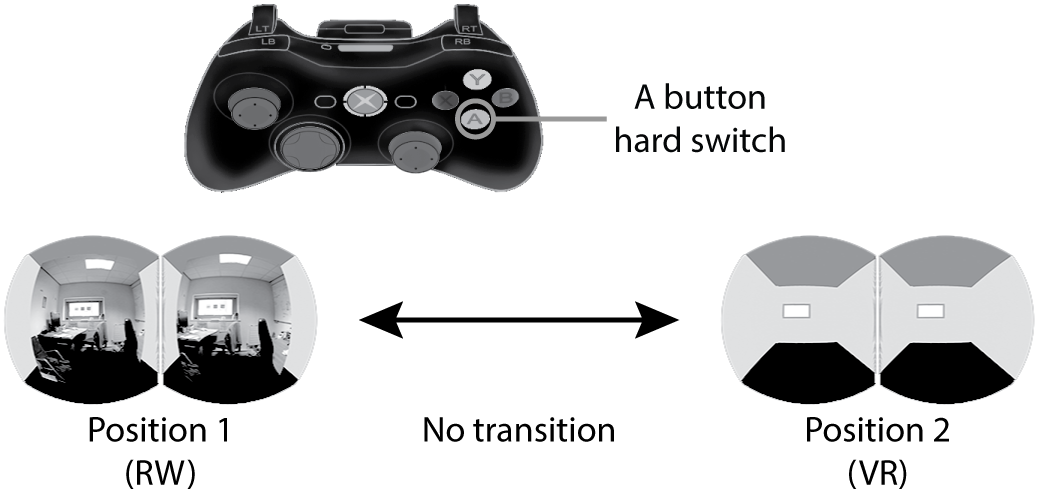
\includegraphics[width=0.7\textwidth]{images/switching-hard-with-controller.png}
		\caption{Hard switch.}
		\label{scenario1}
	\end{center}
\end{figure}

\subsection{Switch with linear interpolation}
The user presses \& holds the \texttt{[B]} button on the controller to switch the visual stimuli displayed by the HMD from RW to VR. When the \texttt{[B]} button is released, the visual stimuli displayed by the HMD switch back from VR to RW. This switch fades between RW \& VR  visual stimuli using linear interpolation on the opacity of the game objects that the webcam feeds are rendered upon. Figure \ref{scenario12} illustrates this scenario.

\begin{figure}[h]
	\begin{center}
		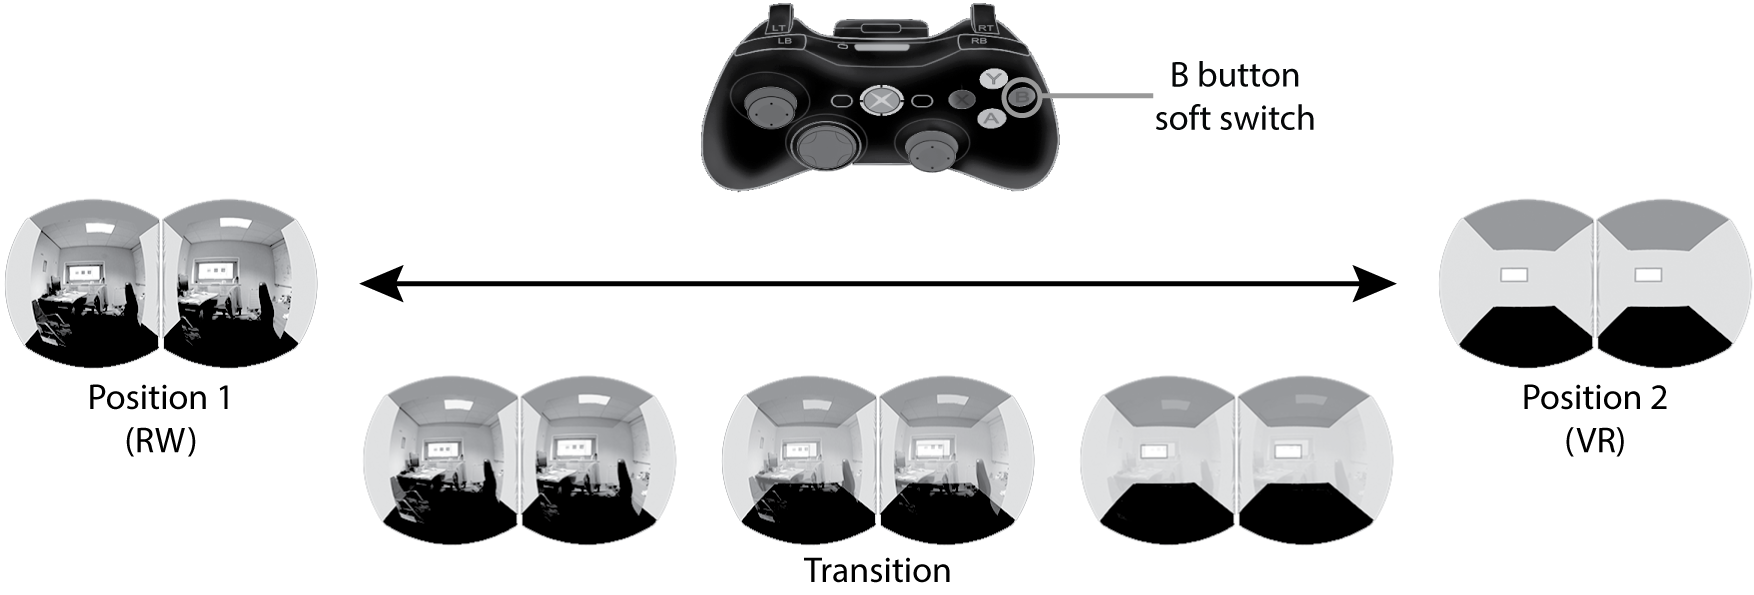
\includegraphics[width=\textwidth]{images/switching-soft-with-controller.png}
		\caption{Switch with linear interpolation.}
		\label{scenario12}
	\end{center}
\end{figure}

\subsection{Analogue selectable opacity}
The user pulls the right analogue trigger (\texttt{[RT]}) on the controller, where the position of the trigger maps directly to the opacity of the game objects that the webcam feeds are rendered upon. The user can choose to stop at any intermediary position that suits their needs, keeping the level of opacity of the webcam feeds at that position, as well as controlling the rate at which the visual stimuli from the RW environment fade (by changing how quickly they change their depression of the trigger). Pulling the trigger all the way in displays only visual stimuli from the VR environment, while releasing it completely displays only visual stimuli from the RW environment. The number of intermediary positions is limited only by the resolution of the trigger \& the encoding of the value.

This method allows the user to superimpose VR visual stimuli upon RW visual stimuli. This is similar, but not identical, to AR, as instead of displaying a small number of virtual objects upon the user's view of their RW environment, a complete VR environment is superimposed upon the user's view of their RW environment. Figure \ref{scenario2} illustrates this scenario.

\begin{figure}[h]
	\begin{center}
		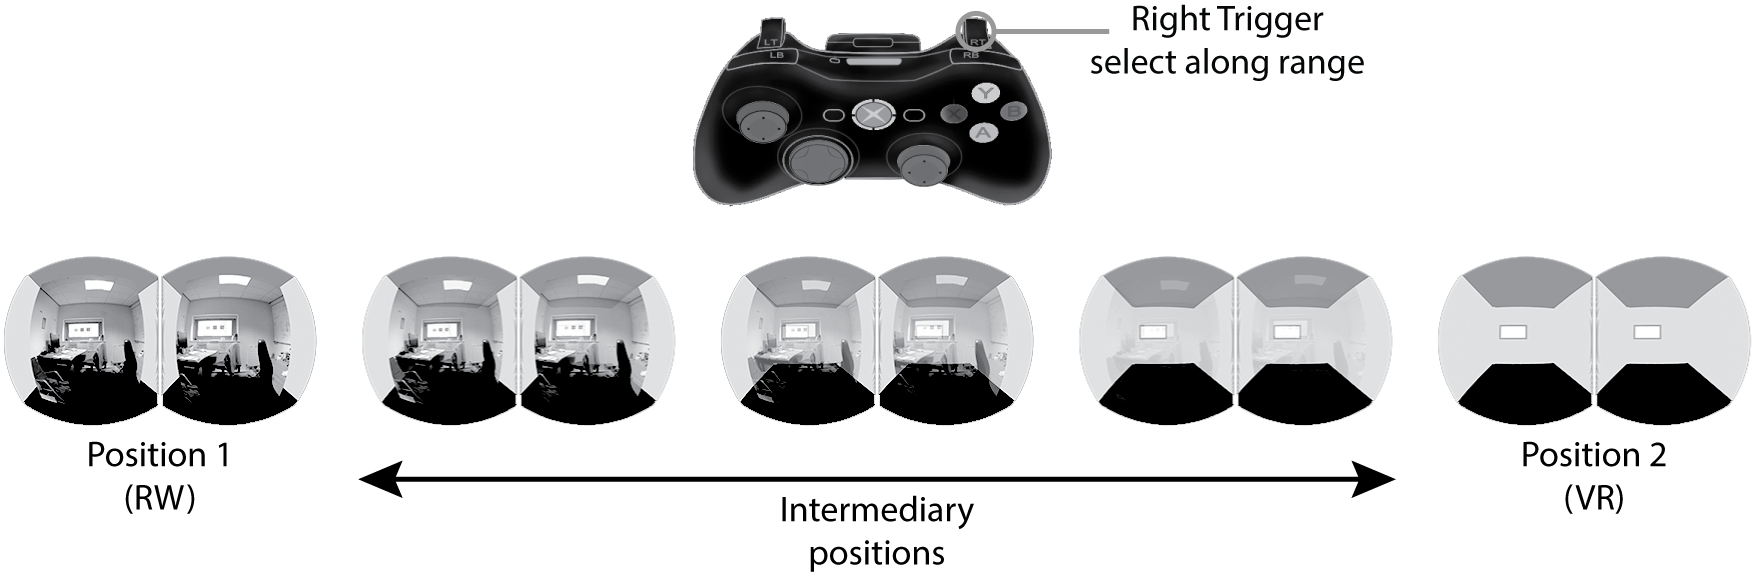
\includegraphics[width=.9\textwidth]{images/switching-analogue-with-controller.png}
		\caption{Analogue selectable opacity.}
		\label{scenario2}
	\end{center}
\end{figure}

\subsection{Periodic hard switches}
\label{subsub-periodic}
Independent or in addition to any of the previous scenarios, the visual stimuli displayed by the HMD switch from RW to VR at a set interval \& for a set amount of time. For example, every 3 seconds the stimuli switch from RW to VR for 0.2 of a second before switching back from VR to RW. Any user triggered transitions cause the interval timer to be reset, such that an `automated' switch will never occur after less time from a user triggered switch than the set interval. Automated transitions are disabled whilst \texttt{[RT]} is at all depressed. Figure \ref{scenariotimed} illustrates this scenario, where \texttt{i} represents the interval between switches \& \texttt{d} represents the duration of the switch from RW to VR.


\begin{figure}[h]
	\begin{center}
		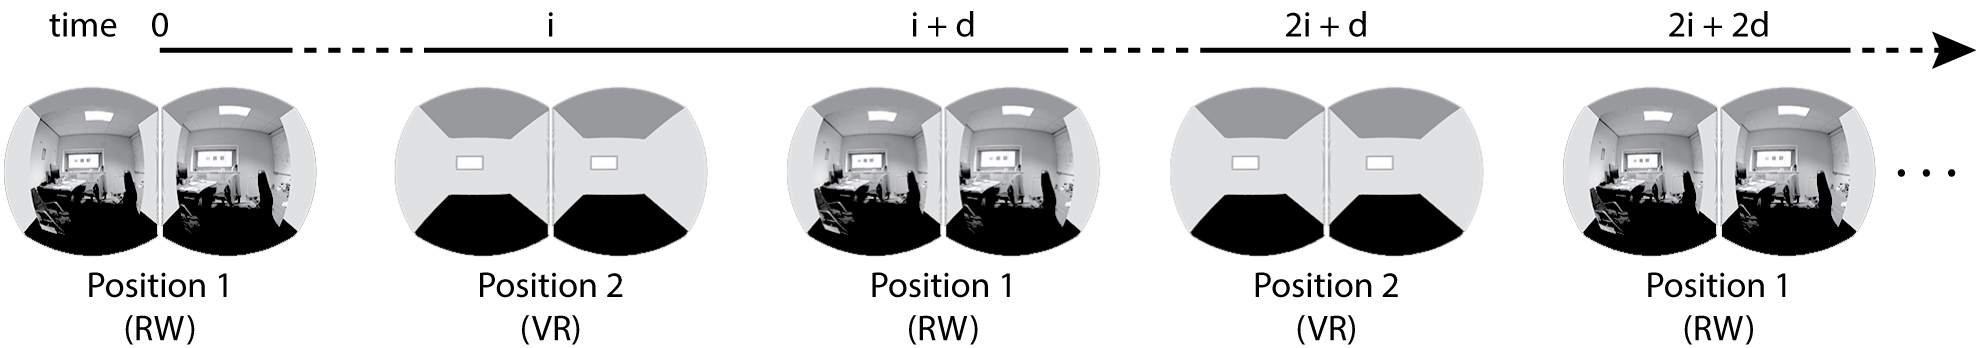
\includegraphics[width=\textwidth]{images/timed-switch.png}
		\caption{Periodic hard switches.}
		\label{scenariotimed}
	\end{center}
\end{figure}


\newpage

\subsection{Reduced maximum opacity}
\label{subsub-baseopacity}
Independent or in addition to any of the previous scenarios, the maximum opacity of the game objects that the webcam feeds are rendered upon is reduced, such that the `default' position at which a transition has not been triggered (either by a button press, trigger movement or by a periodic switch) displays VR superimposed upon RW. Figure \ref{scenariobaseopacity} illustrates this scenario in combination with a hard switch (from section \ref{sub-hardswitch}) in which the user triggers hard switches between the default position of a superimposition of VR upon RW \& a position where only VR stimuli are present.

\begin{figure}[h]
	\begin{center}
		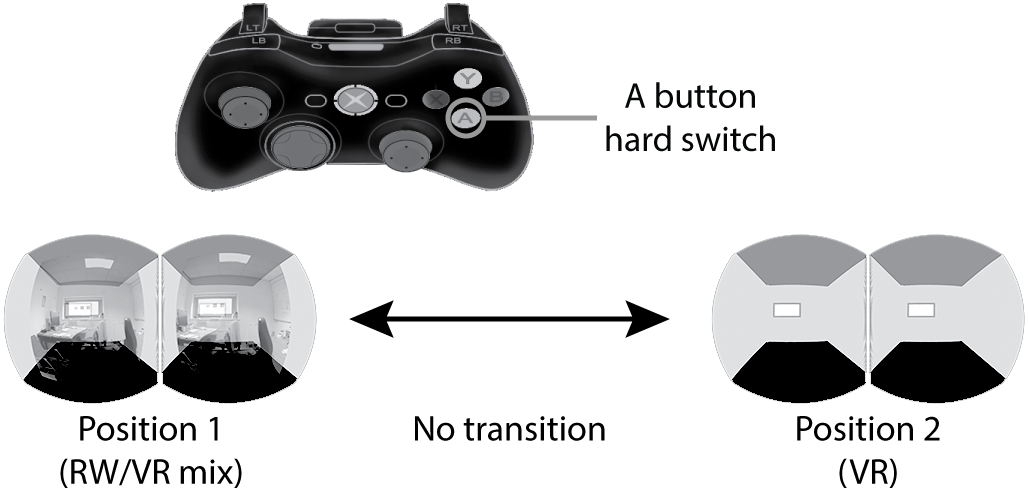
\includegraphics[width=0.7\textwidth]{images/base-opacity-hard-switch.png}
		\caption{Hard switch from reduced maximum opacity.}
		\label{scenariobaseopacity}
	\end{center}
\end{figure}

%=========================================================================================================
%=========================================================================================================

\section{Experimental Task \& Setting}
For these experiments, the HMD is worn upon the head of the participant \& is connected to the laptop computer, battery pack \& wireless receiver worn in a satchel. The smartphone is held in the left hand \& the Xbox controller is held in the right hand (all of the buttons \& triggers used for these experiments are on the right hand side of the controller, designed to be activated with only the right hand).

A task similar to that employed in the first investigation (see section \ref{investigation1} will be employed, encouraging participants to encounter multiple different scenarios of moving, remaining stationary, etc.


%=========================================================================================================


%\textit{Two different buildings have been prepared for use with the Mirrorshades platform, with VR environments constructed \& the IndoorAtlas IPS deployed. The first is a modern building accompanied by a VR environment that closely depicts it in the present day. The second is a historic building accompanied by a VR environment that differs markedly from the present day, by depicting its state a point hundreds of years in the past.}

%\textit{In the first, participants will be given a simple task to complete which will encourage them to engage with the VR environment even though it presents a similar view to their RW environment. In the second scenario, participants will be prompted to engage in more free form exploration of their environments, comparing \& contrasting the markedly different VR environment with what they see around them in their RW environment.}

%\subsection{Jack Cole Building}
%The School of Computer Science Jack Cole building at St Andrews is a modern building, built in 2004. The VR environment accompanying the building is a fairly close representation of the building as it stands today. Figure \ref{jc_layout} shows the layout of the building \& the path that IndoorAtlas has been prepared for.

%There are four coloured panels (red, green, blue \& yellow) situated within the VR building upon walls, floor \& ceiling. Participants will be asked to remember in what order these panels are seen as they walk a lap of the building. This task is designed to encourage participants to switch between RW \& VR visual stimuli, even though the VR visual stimuli are very similar to those of the RW environment. This scenario is also intended to encourage participants to keep moving, rather than stopping at \& starting.

%\begin{figure}[h]
%	\begin{center}
%		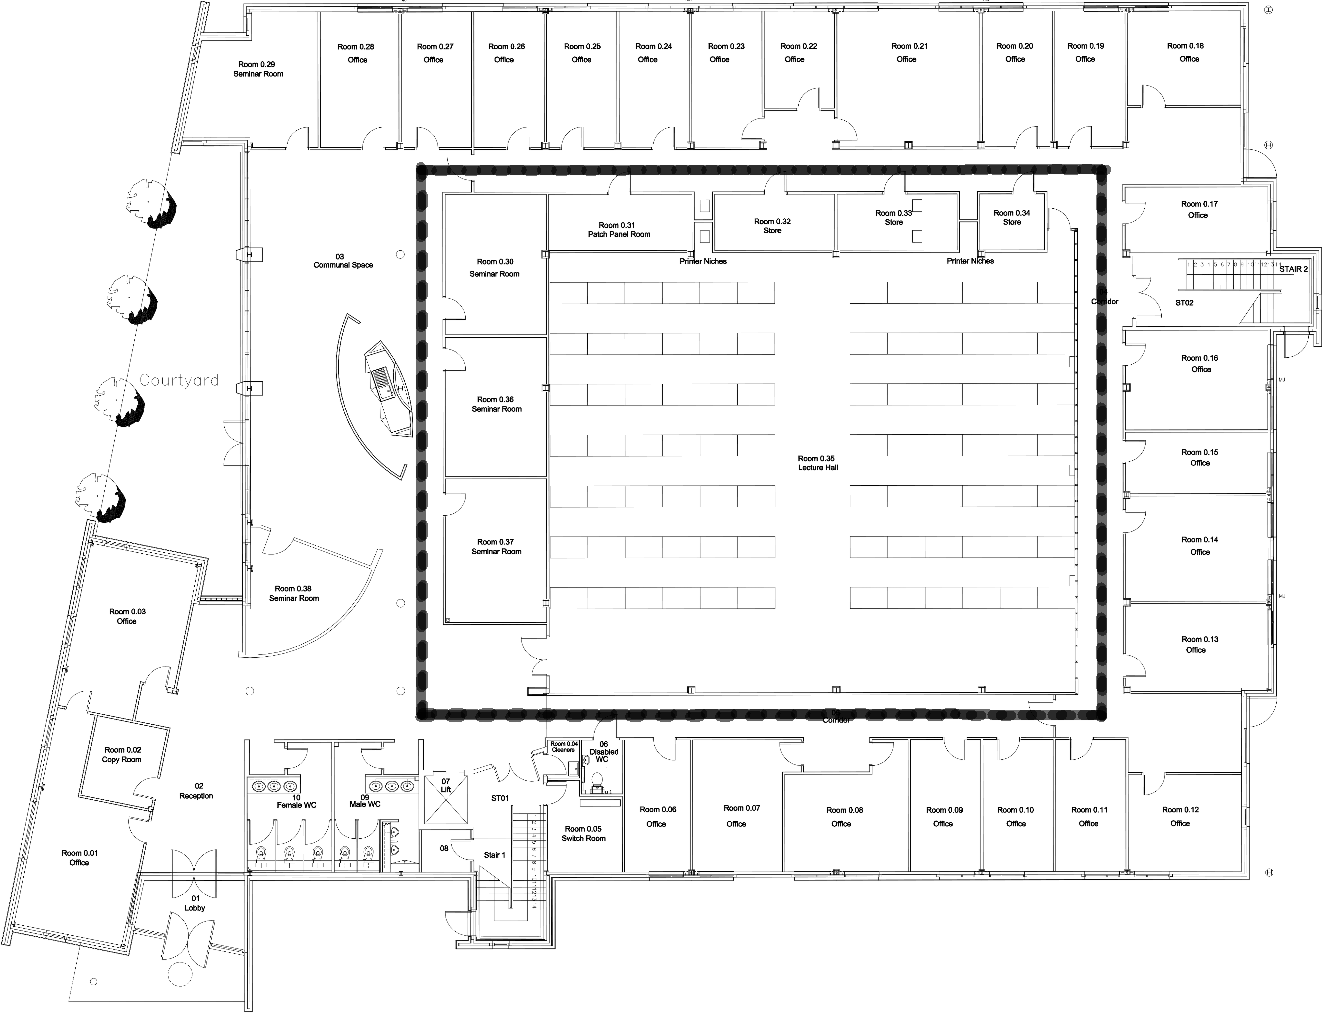
\includegraphics[width=0.7\textwidth]{images/JC_layout.png}
%		\caption{Floor plan of Jack Cole building, with IPS route.}
%		\label{jc_layout}
%	\end{center}
%\end{figure}

%=========================================================================================================
%=========================================================================================================

\section{Evaluation}
%*** explain why we need both Quantitative & Qualitative data?

%What transition styles are preferred in what situations?
%What affects which transition styles are preferred (eg what are the 'situations')?

Evaluating users' preferences toward different methods of transitioning between visual stimuli in different situations pertains to studying their reactions \& responses to ascertain the effect upon their focus of attention, concepts which are largely psychological in nature \& highly subjective~\cite{Ijsselsteijn2001}. Thus, subjective measures will produce the bulk of the data for evaluation. However, objective data will also be collected \& cross referenced with the subjective data in attempts to support or contradict any relationships that are identified.

It is hypothesized that a manner of transitioning between visual stimuli which results in a less severe BIP will be preferable to a manner of transitioning which results in a worse BIP. As focus in the Waterworth model is most closely related to presence in the VR literature~\cite{Waterworth2001}, one of the subjective measures that will be used in this evaluation will be an established presence measure, to try to capture the behaviour of the user's position upon the focus axis.

\subsection{Subjective Quantitative - Post-Task Questionnaire}
After completing the task, participants will respond to the Igroup Presence Questionnaire (IPQ)~\cite{Schubert2001} (see appendix \ref{ipqitems} for the items of the IPQ) which will provide subjective quantitative insight into their experiences with the system, in particular in relation to their position upon the focus axis of the combined model. The IPQ represents a useful questionnaire for evaluation of users' subjective experiences of using the Mirrorshades platform because its terms, especially in the `spatial involvement' scale, question about the RW environment in a manner that does not explicitly present it as a `distraction' from the VR interaction as many other presence questionnaires do.
%examples of other presence questionnaires that present RW stimuli as 'distractions'?

%citation for the components being independent
%The IPQ consists of one general item (G), five items in the `spatial presence' (SP) scale, four items in the `involvement' scale (INV) \& four items in the `realness' scale (REAL). For the purposes of this study, all of the REAL items save REAL2 will be omitted from the questionnaire. The REAL items are primarily concerned with eliciting how `real' participants considered the virtual environment to be. These questions are useful for traditional VR experiences where the user is encouraged to suspend belief \& believe the VR environment they are perceiving to be `real' (the same experiences for which RW stimuli are usually considered a `distraction'). The Mirrorshades platform, however, is less concerned with convincing participants that a VR environment is real \& is more concerned with the juxtaposition of VR \& RW environments.
%It is believed that the other REAL questions will get the participants thinking about the wrong things & hamper their responses when talking about XR

%hypothesis
Whilst a traditional VR experience would hope to elicit high SP1 \& SP4 results combined with low INV1 \& INV3 results, Mirrorshades participants are expected to report high SP1 \& SP4 combined with \textit{high} INV1 \& INV3. The results from participants in this investigation will be compared against those who partook in a `traditional' VR experience wherein RW stimuli were considered a distraction.

% *** But what about the factor analysis, what effect does removing the REAL component have on that?

\subsection{Subjective Qualitative - Interview}
A structured interview will be performed after the IPQ has been completed.

\subsection{Objective Quantitative - Automatic Data Logging}
The Unity app logs the following quantitative data each frame to a tab separated variable (\texttt{.tsv}) file;

\begin{itemize}
	\item \texttt{<frame number>}
	\item \texttt{<timestamp>} - according to the laptop's internal clock
	\item \texttt{<original\_position>} - the position as a Unity \texttt{Vector3} where the user begins the experiment
	\item \texttt{<position>} - the position as a Unity \texttt{Vector3} where the user is on this frame
	\item \texttt{<delta\_x>} \& \texttt{<delta\_z>} - the difference in the \texttt{x} \& \texttt{z} axes between \texttt{<original\_position>} \& \texttt{<position>} on this frame
	\item \texttt{<left\_rotation>} \& \texttt{<right\_rotation>} - the orientations as Unity \texttt{Quaternion} of the two Unity camera game objects
	\item \texttt{<base\_oapcity>} - the maximum opacity of the game objects upon which the webcam feeds are rendered (see section \ref{subsub-baseopacity})
	\item \texttt{<left\_opacity>} \& \texttt{<right\_opacity>} - the opacity on this frame of the game objects upon which the webcam feeds are rendered
	\item \texttt{<auto\_tick>} - whether a periodic switch is in progress (see section \ref{subsub-periodic})
	\item \texttt{<auto\_duration>} \& \texttt{<auto\_spacing>} - the interval \& duration values of the periodic hard switching
	\item \texttt{<framerate>} - an estimate of the current frame rate (frames per second)
	\item \texttt{<A\_button>}, \texttt{<B\_button>} \& \texttt{<right\_trigger>} - the current values of these inputs on the controller
\end{itemize}

\vspace{4mm}

An example line of this output;

\begin{center}
	\texttt{420	08-05-2014 12-34-36-257	(3.4, 1.0, -8.3)	(0.3, 1.0, -8.3)	3.153522	0.0001955032	(-0.1, -0.7, -0.1, 0.7)	(-0.1, -0.7, -0.1, 0.7)	1	1	1	False	0	0	39.57977	False	False	0}
\end{center}

These data are expected to reveal relationships between various different metrics \& the choice of transition methods. For example, it is expected that participants will perform short transitions to VR or transitions to a mix of RW \& VR when moving \& perform longer transitions to VR when stationary. This kind of relationship will support or contradict the subjective data collected through questionnaire \& interview.

%*** SUS?

\subsection{Objective Qualitative - Video Recording}
%*** talk about not prompting them with 'think aloud' vs prompting (where prompting changes their responses)
During experiments, the video feed being displayed by the HMD will be recorded \& the user will be recorded using a video camera (both video \& audio). The video of the HMD graphics will be used in comparison with the quantitative data, while the video \& audio recording of the user will provide objective insight into their behaviour.

%\subsection{Evaluation Techniques}
%These data will make it possible both to statistically assess preferred switching/fading methods, but also to infer any relationships between different switching/fading methods \& other behaviours: for example, a certain style of switching/fading may frequently appear after a period of movement, but rarely when the participant is stationary.

%\section{Hypothesis}
%Null hypothesis includes things like;
%\begin{itemize}
%	\item different transitions do not alter user `enjoyment'
%	\item users will not prefer one transition over another
%	\item choice of transition will have no effect on circumstances/scenarios
%	\item users will not move head less when walking
%	\item users will not spend less time in virtual when walking
%	\item etc.
%\end{itemize}

%=========================================================================================================
%=========================================================================================================

\section{Preliminary Results}
Figure \ref{plot} shows three of the fields of the automatic data logging, \texttt{<left\_opacity>}, \texttt{<left\_rotation>} \& the sum of \texttt{<delta\_x>} \& \texttt{<delta\_z>}, plotted against \texttt{<frame\_number>} for a set of data collected during a preliminary test. A precursory glance at this plot reveals that certain relationships can be gleaned between these series;

\begin{itemize}
	\item Where the user is standing still (no change in the y axis for position, blue line) there is more marked head movement (more change in the y axis for orientation, green line); for example, frames 1100-1650, 2550-2950 \& 4500-5000.
	\item Where the user is moving at a steady speed (steady climb or fall in y of position, blue line) we see the user switching to a semi opaque virtual feed rather than complete transitions to 100\% virtual which appear to be more common when standing still; for example, frames 500-700, 3000-3300 \& 4000-4100.
\end{itemize}

\pagebreak
\begin{landscape}
\vspace*{\fill}
\begin{figure}[h]
	\thispagestyle{empty}
	\begin{center}
		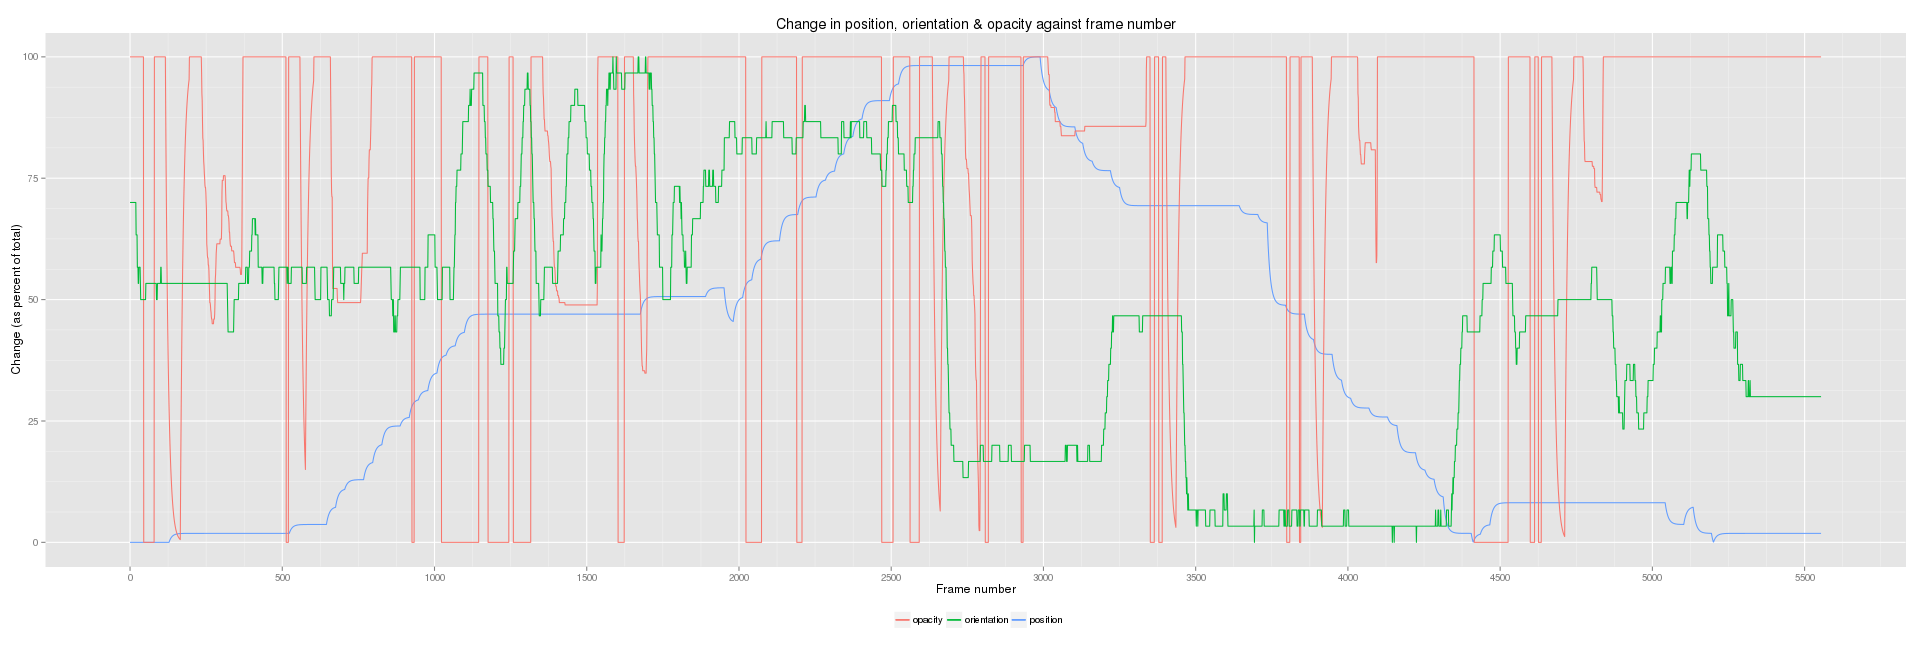
\includegraphics[width=\linewidth]{images/graph.png}
		\caption{Plot of a subset of example objective quantitative data logged by the Unity application.}
		\label{plot}
	\end{center}
\end{figure}
\vspace*{\fill}
\end{landscape}
\pagebreak

\appendix

\chapter{IPQ Items}

\label{ipqitems}

\begin{flushleft}

G1: In the computer generated world I had a sense of ``being there''.

\vspace{4mm}

%Spatial presence

SP1: Somehow I felt that the virtual world surrounded me.

\vspace{4mm}

SP2: I felt like I was just perceiving pictures.

\vspace{4mm}

SP3: I did not feel present in the virtual space.

\vspace{4mm}

SP4: I had a sense of acting in the virtual space, rather than operating something from outside.

\vspace{4mm}

SP5: I felt present in the virtual space.

\vspace{4mm}

%Involvement

INV1: How aware were you of the real world surrounding while navigating in the virtual world? (i.e. sounds, room temperature, other people, etc.)?

\vspace{4mm}

INV2: I was not aware of my real environment.

\vspace{4mm}

INV3: I still paid attention to the real environment.

\vspace{4mm}

INV4: I was completely captivated by the virtual world.

%REAL

\vspace{4mm}

REAL1: How real did the virtual world seem to you?

\vspace{4mm}

REAL2: How much did your experience in the virtual environment seem consistent with your real world experience?

\vspace{4mm}

REAL3: How real did the virtual world seem to you?

\vspace{4mm}

REAL4: The virtual world seemed more realistic than the real world.

\end{flushleft}

\bibliographystyle{unsrt}
\bibliography{bib}

\end{document}